\chapter{Экспериментальное обоснование метода неконтролируемого предобучения}

В данной главе приводится практическое обоснование теоретических результатов, описанных в главе 2, а именно, результаты сравнительного анализа методов предобучения и алгоритма редуцирования весовых коэффициентов нейросетевых моделей.

Для оценки эффективности предлагаемых методов применяются известные выборки данных, используемые для апробации подходов в области машинного обучения:
% Представленные результаты получены на известных выборках компьютерного зрения, используемых для оценки эффективности выбранных архитектур и подходов:
\begin{easylistNum}
    & выборка MNIST, представляющая собой набор из 70.000 черно-белых изображений рукописных цифр размерностью 28Х28 пикселей, представленных в виде одномерных векторов данных \cite{mnist};
    & выборка CIFAR-10, представляющая собой набор из 60.000 цветных изображений объектов 10 различных классов размерностью 32Х32 пикселя \cite{krizhevsky2009learning};
    & выборка CIFAR-100, представляющая собой набор из 60.000 цветных изображений объектов 100 различных классов размерность 32Х32 пикселя \cite{krizhevsky2009learning}.
\end{easylistNum}

Приводятся результаты экспериментальных исследований, полученных для задач сжатия данных, распознавания образов и редуцирования параметров ГНС.

Исходный код реализованных методов предобучения и редуцирования ИНС приводится в приложении \ref{app:a}.

%\section{Используемое программное и аппаратное обеспечение}

%Выполнение экспериментов с использованием выборок большого размера занимает достаточно продолжительное время. Эта проблема была решена проведением расчетов с использованием видеокарт nVidia, поддерживающих технологию CUDA (нами использовались ускорители A100 или V100, доступные при использовании сервиса Google Colab \cite{googlecolab}). Существуют другие способы ускорения расчетов, производимых при обучении нейронной сети, например, использование вычислительных кластеров \cite{n16}.

\section{Сжатие данных}

Для первоначальной оценки эффективности предлагаемого подхода предобучения глубокой нейронной сети, были проведены вычислительные эксперименты на искусственном наборе данных $\boldmath{x}$, лежащем на одномерном многообразии (спиральная петля), погруженном в трехмерное пространство \cite{n11} и генерируемом равномерно распределенным параметром $t \in [-1, 1]$:

\begin{equation*}
	\begin{cases}
		x_1=\sin(\pi t) + \mu\\
		x_2=\cos(\pi t) + \mu\\
		x_3=t + \mu
	\end{cases}
\end{equation*}
где $\mu$ -- Гауссов шум со средним 0 и стандартным отклонением 0.05.

Для проверки предложенного метода, был обучен семислойный автоэнкодер, используя выборку из 1000 примеров. Глубокий автоэнкодер показан на рисунке \ref{fig:autoencoder}. Мы использовали логистические функции активации для всех слоев нейронной сети, за исключением среднего слоя (<<узкого места>>). На этом слое использовалась линейная функция активации.

\begin{figure}[ht]
	\centering
	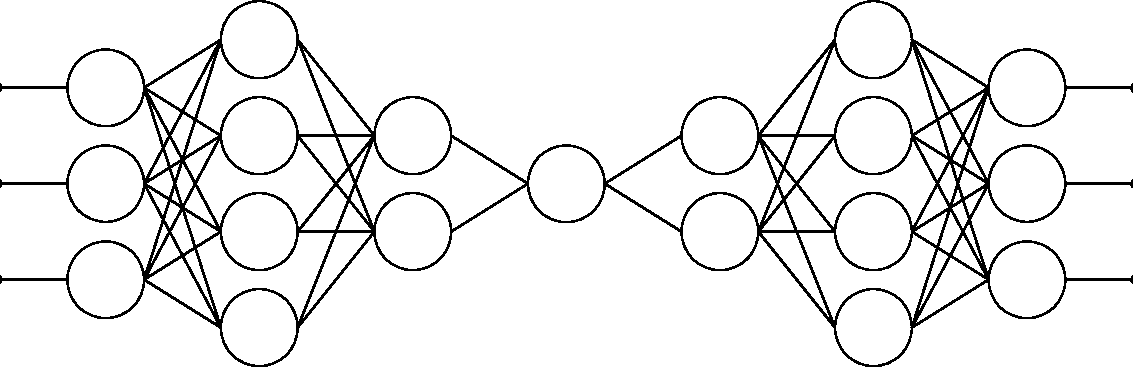
\includegraphics[width=16cm]{man-source/images/ch3/pic3-5.pdf}
	\caption{Глубокий автоэнкодер}
	\label{fig:autoencoder}
\end{figure}

Результаты обучения показаны в таблице \ref{table:data_compressing}. Здесь MSE -- среднеквадратичная ошибка на выборке обучения, MS -- среднеквадратичная ошибка на тестовой выборке для проверки обобщающей способности сети. Количество примеров в тестовой выборке -- 1000. Скорость обучения $\alpha$ -- 0.1 для классического метода обучения и 0.5 для REBA для всех экспериментов.

			\begin{table}[h]
				\caption{Сравнение методов предобучения (сжатие)}								\label{table:data_compressing}
				\centering
				\begin{tabular}{|p{4cm}|p{3cm}|p{2cm}|p{2cm}|}
					\hline
					%					\hline\noalign{\smallskip}
					Метод & CD-k & MSE & MS \\
					%					\noalign{\smallskip}
					%					\hline
					%					\noalign{\smallskip}
					\hline
					C-RBM & 1  & 0,699 & 0,886 \\
                        \cline{2-4}
					& 5  & \textbf{0,710} & \textbf{0,932}\\
                        \cline{2-4}							
					&	10 & 0,689 & 0,916\\
					\cline{2-4}
                        &	15 & \textbf{0,688} & \textbf{0,873}\\ \hline
					REBA& 1  & \textbf{0,673} & \textbf{0,851}\\
                        \cline{2-4}
					& 5  & 0,719 & 0,966\\
                        \cline{2-4}
					&	10 & \textbf{0,677} & \textbf{0,907}\\
                        \cline{2-4}
					&	15 & 0,700 & 0,895 \\						
					\hline
				\end{tabular}			
			\end{table}	

Число эпох предобучения -- 10. Число эпох <<тонкой настройки>> нейронной сети -- 1000. Из полученных результатов видно, что использование метода предобучения REBA позволило улучшить обобщающую способность глубокого автоэнкодера для случаев CD-1 и CD-10. На рисунках \ref{f:15} и \ref{f:16} изображены оригинальные данные, на которых производилось обучение, и восстановленные из одного нелинейного компонента, используя тестовые данные. Как можно видеть, автоэнкодер восстанавливает данные из одного нелинейного компонента с хорошей точностью.

\begin{figure}[h]
	\begin{center}
		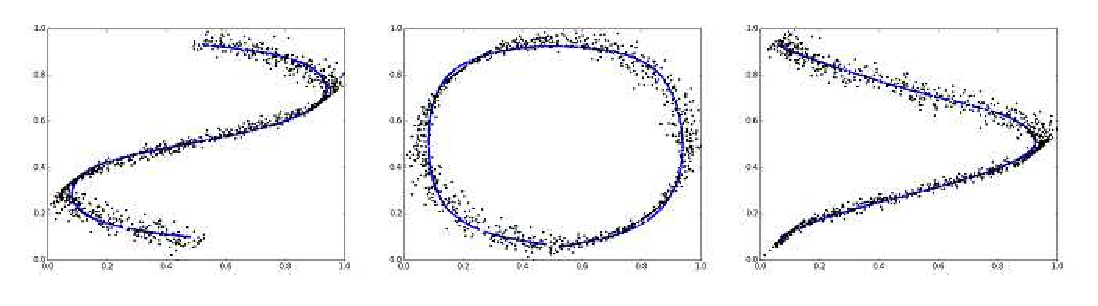
\includegraphics[width=160mm]{man-source/images/ch3/pic3-6.pdf}
		\caption{2D-изображения оригинальных и реконструированных данных}				
		\label{f:15}
	\end{center}
\end{figure}

\begin{figure}[h!]
	\begin{center}
		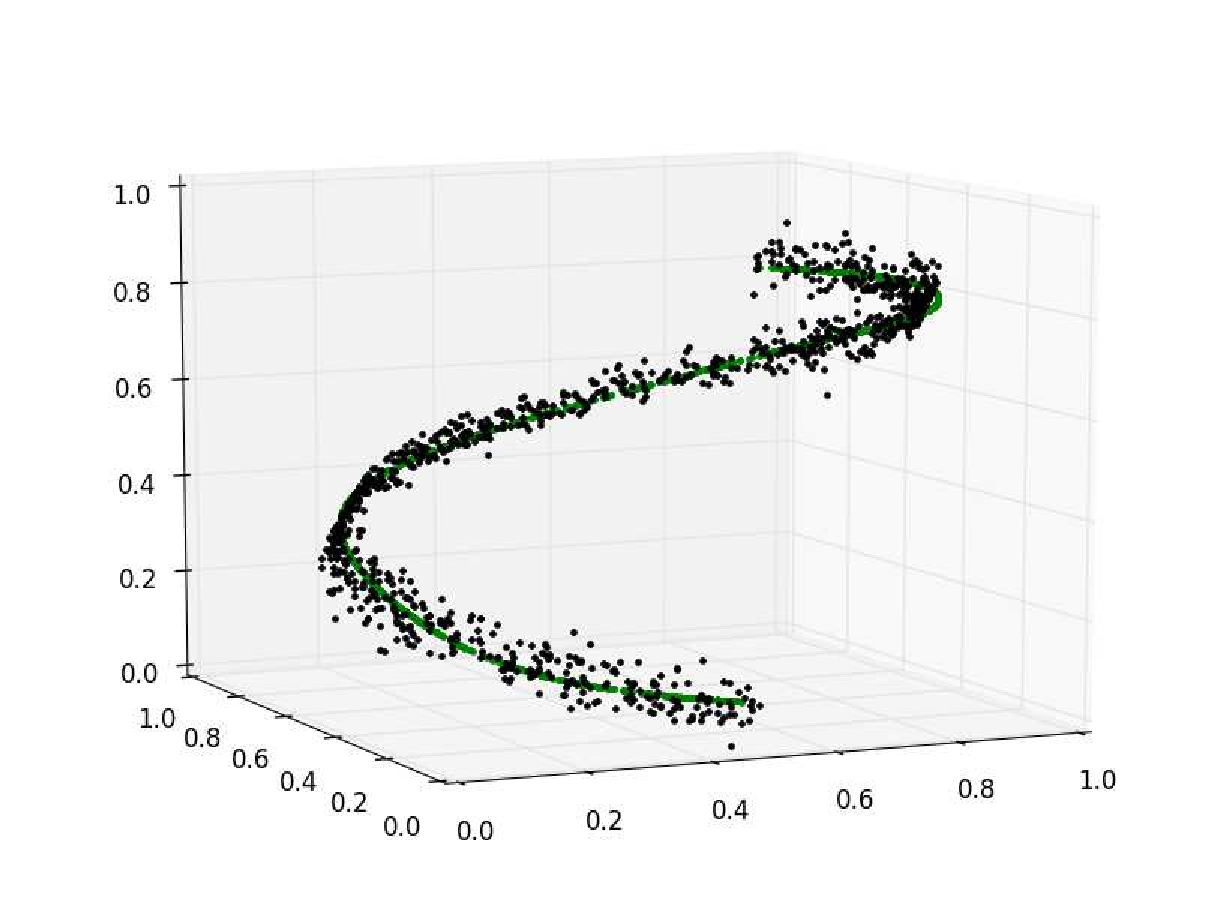
\includegraphics[width=120mm]{man-source/images/ch3/pic3-7.pdf}
		\caption{3D-изображение оригинальных и реконструированных данных}				
		\label{f:16}
	\end{center}
\end{figure}

% \section{Распознавание образов}
% \subsection{Ирисы Фишера}

% Рассмотрим решение задачи распознавания образов на примере известной выборки Фишера \cite{Fisher}. Эта выборка была представлена Рональдом Фишером в 1936 году в качестве примера для демонстрации разработанного им метода линейного дискриминантного анализа. Она включает 150 образов ирисов, относящихся к трем различным классам. Каждый образ представляет собой 4-х мерный вектор признаков.

% Отличительная особенность этой задачи в том, что один класс образов является линейно разделимым, в то время как два других -- нет (рис. \ref{fig:irises_visualize}).

% \begin{figure}[h]
% 	\begin{center}
% 		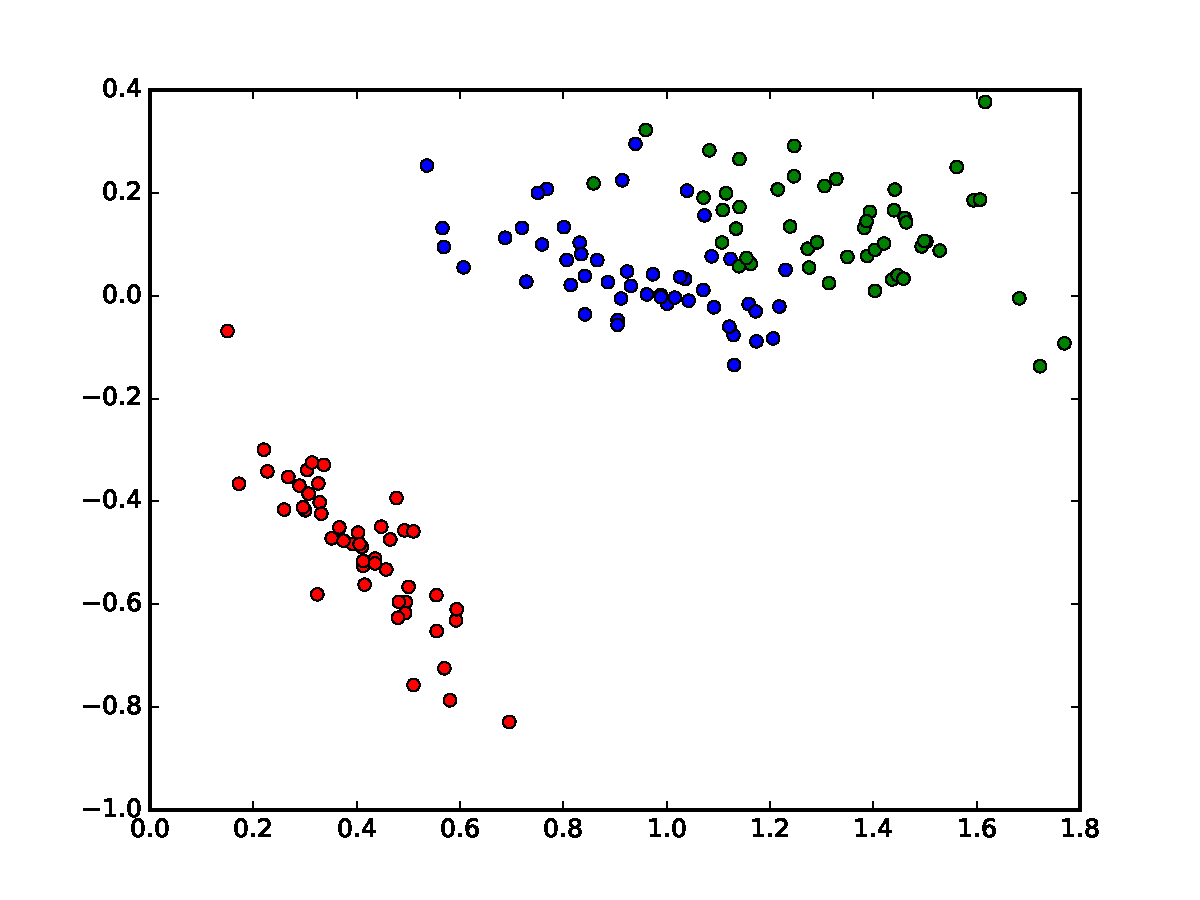
\includegraphics[width=10cm]{man-source/images/ch3/pic3-8.pdf}
% 		\caption{Визуализация образов ирисов Фишера (получена применением PCA)}				
% 		\label{fig:irises_visualize}
% 	\end{center}
% \end{figure}

% Применяя классические подходы кластеризации (например, метод k-средних), можно заметить неприемлемое качество распознавания на границах двух линейно неразделимых классов (рис. \ref{fig:kmeans})

% \begin{figure}[h]
% 	\begin{center}
% 		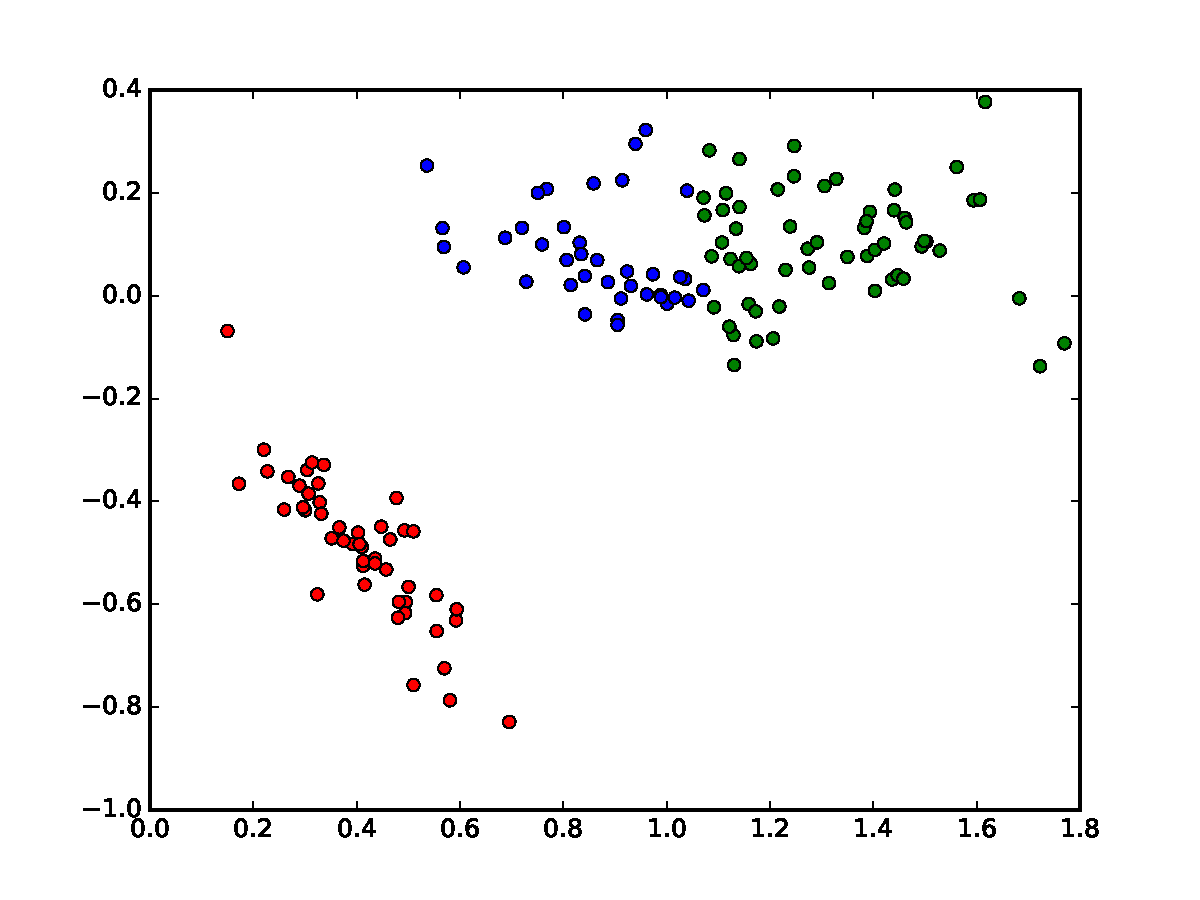
\includegraphics[width=10cm]{man-source/images/ch3/pic3-9.pdf}
% 		\caption{Кластеризация образов ирисов Фишера методом k-средних}			
% 		\label{fig:kmeans}
% 	\end{center}
% \end{figure}

% Обучим глубокую нейронную сеть для классификации образов из выборки Фишера. Для решения этой задачи воспользуемся сетью с архитектурой \textbf{4-32-16-8-3} с сигмоидными функциями активации на каждом обрабатывающем слое. 
% Другие параметры:
% \begin{itemize}
% 	\item Фаза предобучения: скорость -- 0.1 (для REBA 0.4), моментный параметр -- переменный (от 0.5 до 0.9), размер мини-батча - 5, количество эпох обучения каждого слоя -- 50.
% 	\item Фаза обучения: скорость -- 0.05 (с редуцированием, коэффициент 0.99), моментный параметр -- 0.9, размер мини-батча -- 5, количество эпох обучения -- 2000, параметр L2-регуляризации (weight decay) -- 0.00001.
% \end{itemize}

% После обучения нейронной сети нами была достигнута совокупная ошибка распознавания 99,33\%. Таким образом, неправильно распознанным остался только один образ из всей выборки (см. рис. \ref{fig:fisher_irises_results}).

% \begin{figure}[h]
% 	\begin{center}
% 		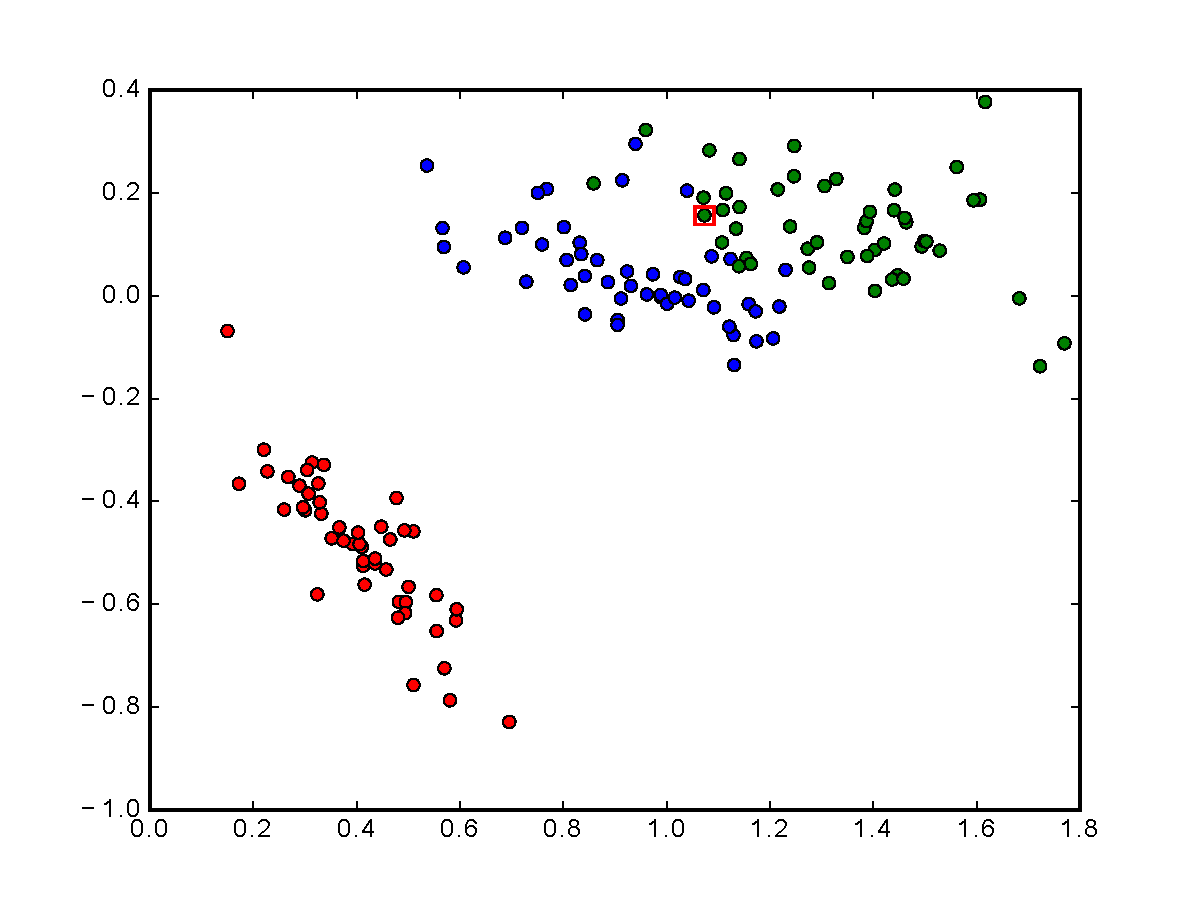
\includegraphics[width=12cm]{man-source/images/ch3/pic3-10.pdf}
% 		\caption{Результат работы обученной глубокой нейронной сети с отмеченным неправильно классифицированным образом}				
% 		\label{fig:fisher_irises_results}
% 	\end{center}
% \end{figure}

% Показательной в данном случае является эволюция среднеквадратичной ошибки после предобучения разными методами и без него (рис. \ref{fig:error_evolution}).

% \begin{figure}[h]
% 	\begin{center}
% 		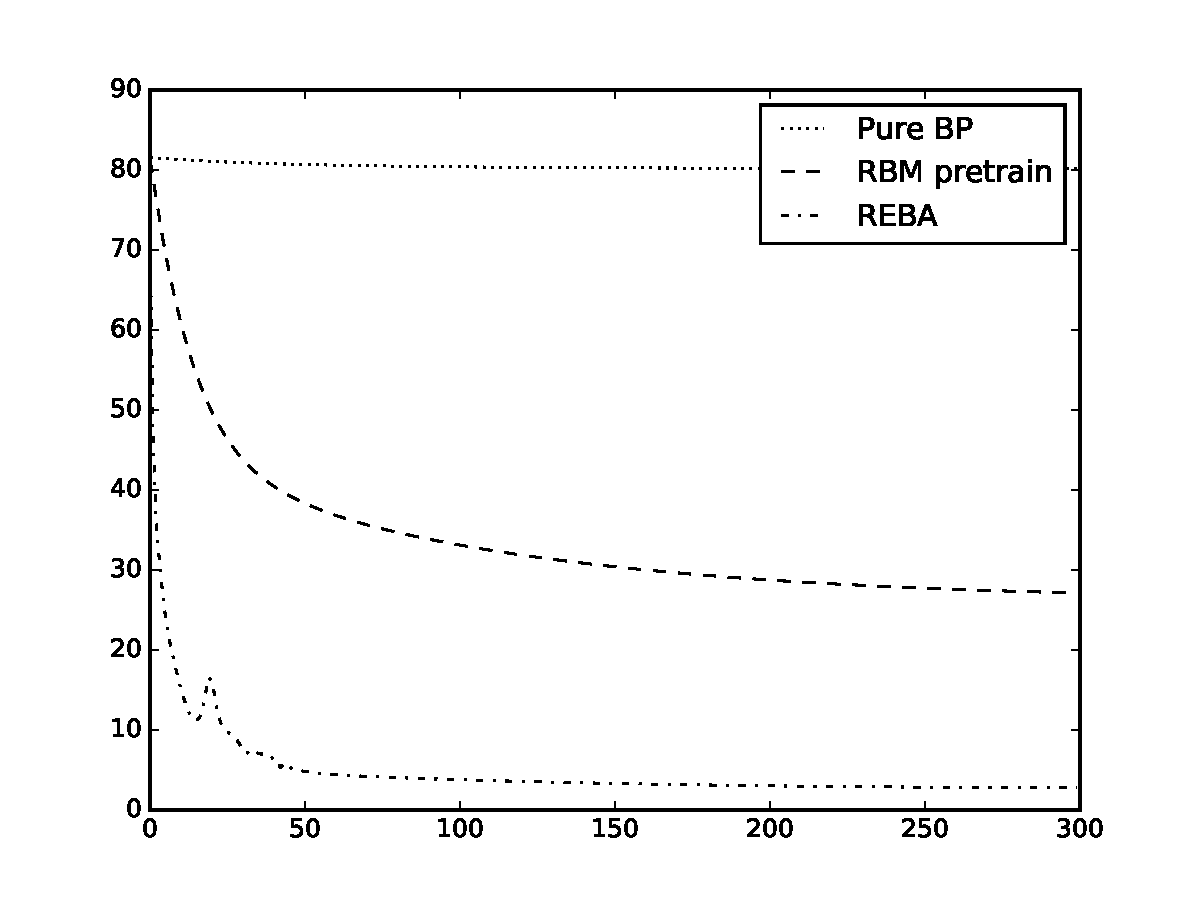
\includegraphics[width=12cm]{man-source/images/ch3/pic3-11.pdf}
% 		\caption{Эволюция ошибок обучения разными методами}	
% 		\label{fig:error_evolution}
% 	\end{center}
% \end{figure}

% Таким образом, предобучение позволяет получить хорошую начальную инициализацию весов и порогов нейронной сети, что делает последующий этап <<тонкой настройки>> методом обратного распространения ошибки значительно более продуктивным.

% \section{Гибридный алгоритм предобучения}

% При обучении нейронных сетей, как поверхностных, так и глубоких архитектур, можно использовать целевые минимизируемые функции разных видов. В главе 1 были приведены основные функции ошибок, часто применяемые на практике (\ref{MSE}, \ref{CE}).

% В различных публикациях исследуется вопрос применения обоих критериев (например, \cite{Golik}, \cite{Zhou}). При этом полученные в \cite{Golik} результаты подтверждают, что обучение классификаторов в соответствии с критерием $E_{CE}$ позволяет найти лучший локальный оптимум, чем с критерием $E_{MSE}$, применение которого приводит к быстрому <<застреванию>> в локальном оптимуме, где градиент стремится к нулю и, как результат, дальнейшее уменьшение ошибки классификации становится невозможным. 

% В \cite{Golik} исследуется вопрос применения гибридного подхода. Начиная с хорошей начальной инициализации, полученной при обучении с критерием $E_{CE}$, дальнейший процесс с $E_{MSE}$ способен дать лучший результат, чем при обучении только с критерием $E_{CE}$. 

% % При этом полученные авторами результаты подтверждают, что если обучение вначале будет вестись в соответствии с правилами по формуле $E_{CE}$, а затем несколько эпох - по формуле $E_{MSE}$, итоговая обобщающая способность сети будет выше, чем при обучении только с использованием $E_{CE}$.

% Таким образом, с учетом ранее доказанных теорем, может быть сформулирован гибридный вариант предобучающего алгоритма.

\section{Распознавание образов}

\subsection{Критерий оценки результатов классификации}

Для оценки качества решения задачи классификации применялся следующий подход. Вначале определялся $k$-тый нейрон, выходное значение которого было максимальным для заданного образа $s$ (данное число соответствует метке класса, получаемого моделью):

\begin{equation}
k_s = \arg \max_j y_j^s
\end{equation}

Затем получившееся значение сравнивалось с эталонными значениями и количество совпадений суммировалось для всех образов:

\begin{equation}
S = \sum_{s=1}^{L} I[k_s = e_s]
\end{equation}
где $I[]$ -- индикаторная функция, $L$ -- общее количество образов из оцениваемого множества, $e_s$ -- эталонное значение, метка класса, соответствующая $s$-тому образу.

Значения индикаторной функции могут быть получены по следующей формуле:

\begin{equation*}
    I[x] = 
    \begin{cases}
        1, & \text{x is True} \\
        0, & \text{x is False}
    \end{cases}
\end{equation*}

Таким образом, общая эффективность на тестовой выборке может быть получена по следующей формуле:

\begin{equation}
\text{Efficiency} = \frac{S}{L} * 100\%
\end{equation}

%Основной задачей при проведении вычислительных экспериментов являлась сравнительная характеристика классического и предложенного подходов для предобучения нейронной сети. 

\subsection{Ирисы Фишера}

Рассмотрим решение задачи распознавания образов на примере известной выборки Фишера \cite{Fisher}. Эта выборка была представлена Рональдом Фишером в 1936 году в качестве примера для демонстрации разработанного им метода линейного дискриминантного анализа. Она включает 150 образов ирисов, относящихся к трем различным классам. Каждый образ представляет собой 4-х мерный вектор признаков.

Отличительная особенность этой задачи в том, что один класс образов является линейно разделимым, в то время как два других -- нет (рис. \ref{fig:irises_visualize}).

\begin{figure}[h]
	\begin{center}
		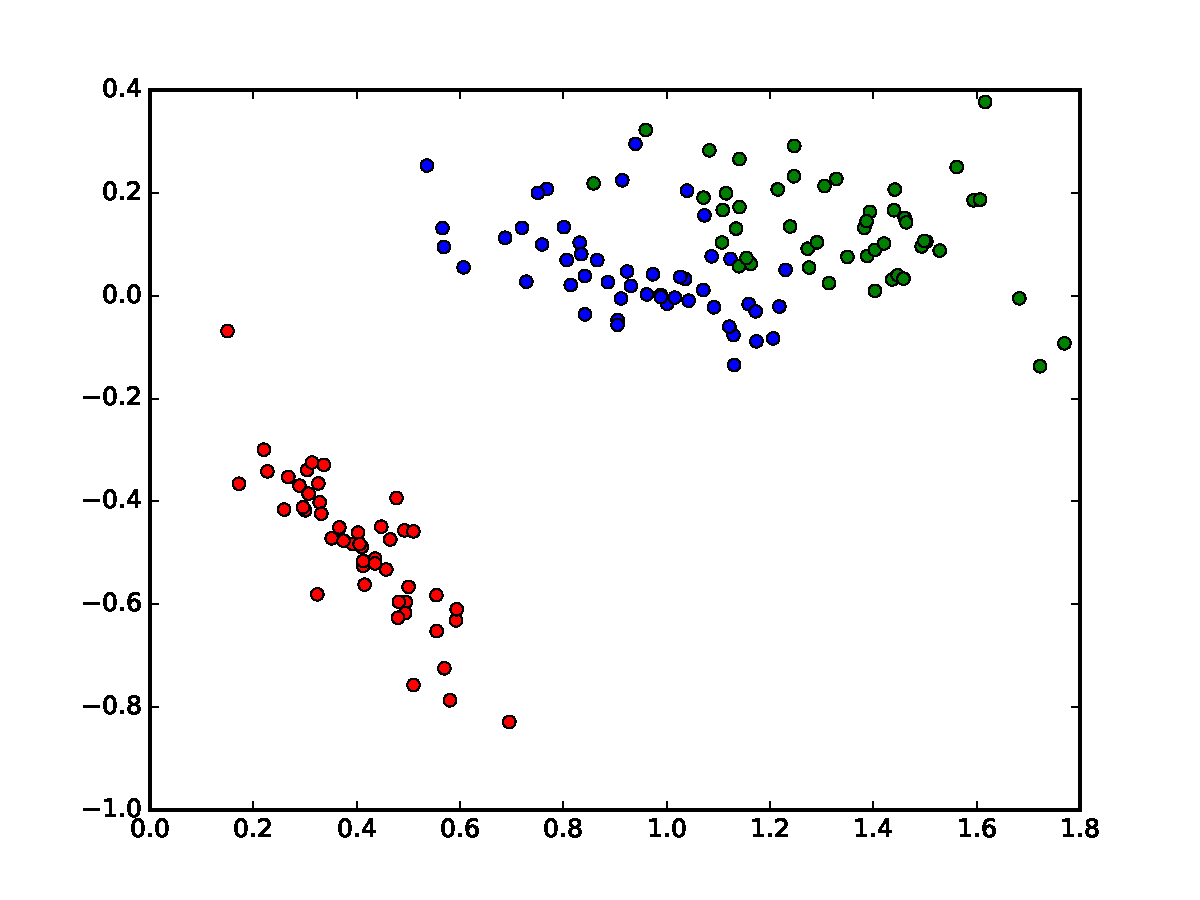
\includegraphics[width=10cm]{man-source/images/ch3/pic3-8.pdf}
		\caption{Визуализация образов ирисов Фишера (получена применением метода PCA)}				
		\label{fig:irises_visualize}
	\end{center}
\end{figure}

Применяя классические подходы кластеризации (например, метод k-средних), можно заметить неприемлемое качество распознавания на границах двух линейно неразделимых классов (рис. \ref{fig:kmeans})

\begin{figure}[h]
	\begin{center}
		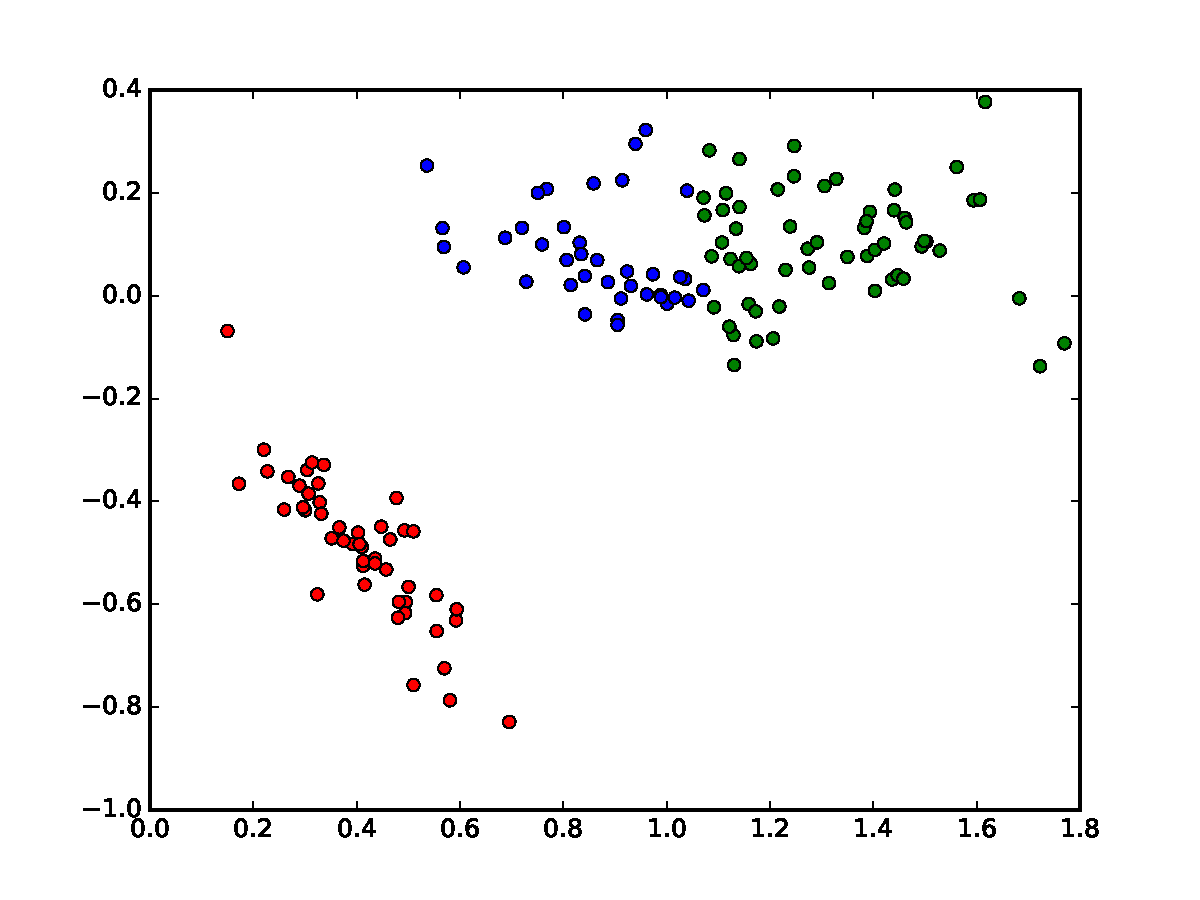
\includegraphics[width=10cm]{man-source/images/ch3/pic3-9.pdf}
		\caption{Кластеризация образов ирисов Фишера методом k-средних}			
		\label{fig:kmeans}
	\end{center}
\end{figure}

Для решения этой задачи была использована сеть с архитектурой \textbf{4-32-16-8-3} с сигмоидными функциями активации на каждом обрабатывающем слое. 
Другие параметры:
\begin{itemize}
	\item Фаза предобучения: скорость -- 0.1 (для REBA 0.4), моментный параметр -- переменный (от 0.5 до 0.9), размер мини-батча - 5, количество эпох обучения каждого слоя -- 50.
	\item Фаза обучения: скорость -- 0.05 (с редуцированием, коэффициент 0.99), моментный параметр -- 0.9, размер мини-батча -- 5, количество эпох обучения -- 2000, параметр L2-регуляризации (weight decay) -- 0.00001.
\end{itemize}

После обучения нейронной сетью была достигнута совокупная ошибка распознавания 99,33\%. Таким образом, неправильно распознанным остался только один образ из всей выборки (см. рис. \ref{fig:fisher_irises_results}).

\begin{figure}[h]
	\begin{center}
		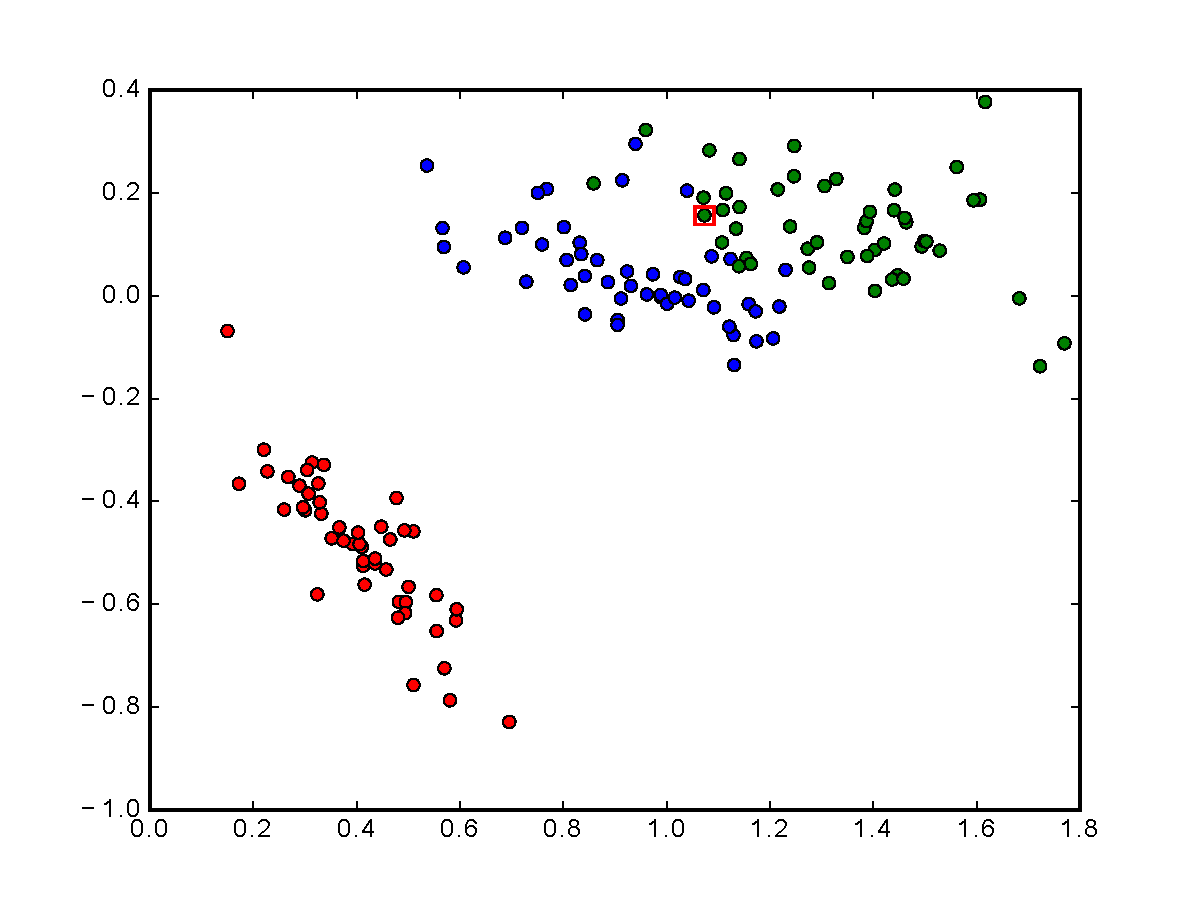
\includegraphics[width=12cm]{man-source/images/ch3/pic3-10.pdf}
		\caption{Результат работы обученной нейронной сети с отмеченным неправильно классифицированным образом}				
		\label{fig:fisher_irises_results}
	\end{center}
\end{figure}

Эволюция среднеквадратичной ошибки после предобучения разными методами и без предобучения изображена на рис. \ref{fig:error_evolution}.

\begin{figure}[h]
	\begin{center}
		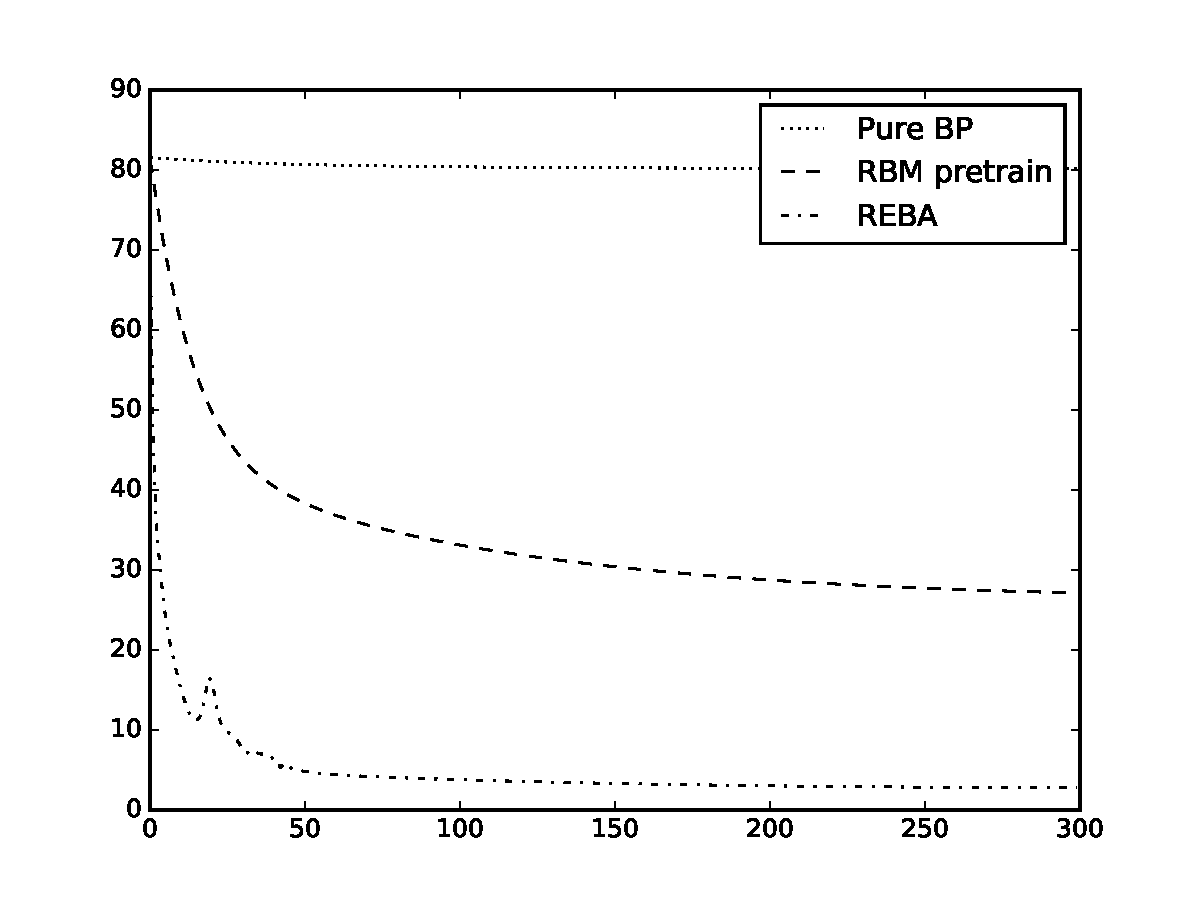
\includegraphics[width=12cm]{man-source/images/ch3/pic3-11.pdf}
		\caption{Эволюция ошибок обучения разными методами}	
		\label{fig:error_evolution}
	\end{center}
\end{figure}

Как видно из представленного графика, предобучение позволяет получить хорошую начальную инициализацию весов и порогов нейронной сети, что делает последующий этап <<тонкой настройки>> методом обратного распространения ошибки более эффективным.

\subsection{Описание выборок}

С практической точки зрения (и в соответствии с объектом исследования) наибольший интерес представляют выборки графических образов.

Задача распознавания графических образов является одной из основных в области компьютерного зрения. В настоящий момент <<золотым стандартом>> выборок, применяемых для оценки эффективности моделей выступают MNIST, CIFAR-10 и CIFAR-100. %На этих выборках уже получены хорошие результаты по достигнутой эффективности моделей. Однако, нужно отметить, что для ряда подходов, для которых получены лучшие результаты при тестировании на данных выборках, используются аугментированные (т.е. измененные данные), которые позволяют значительно увеличить размерность обучающей выборки. Перед нами стояла задача сравнения методов предобучения, без достижения state-of-art результатов для выборок, поэтому методы аугментации данных не применялись.

Выборка MNIST (Mixed National Institute of Standards and Technology database) является классической при тестировании систем распознавания образов, а также широко используемой для обучения и тестирования алгоритмов машинного обучения. Она сформирована как подмножество более крупной оригинальной выборки NIST \cite{mnist}, изображения из которого были дополнительно предобработаны (путем изменения размера и центрирования). 

Выборка MNIST состоит из 60000 образов для обучения и 10000 образов для тестирования. Каждый образ представляет собой изображение цифры размером 28Х28 пикселей в градациях серого цвета. На рис. \ref{fig:mnist_example} изображен фрагмент базы изображений MNIST с наиболее труднораспознаваемыми цифрами.

\begin{figure}[h]
	\begin{center}
		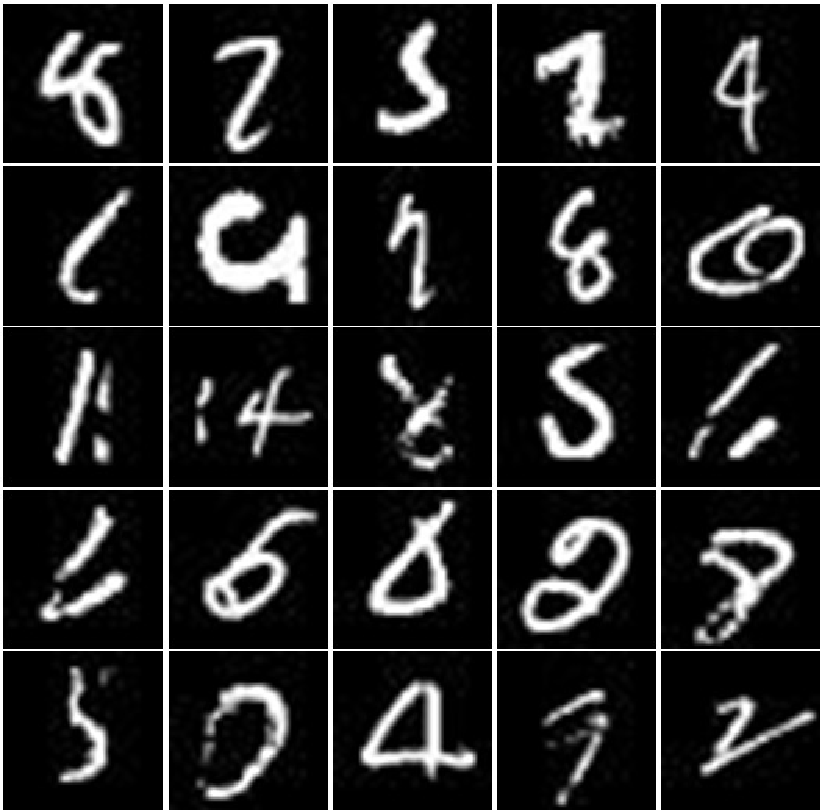
\includegraphics[width=8cm]{man-source/images/ch3/pic3-12.pdf}
		\caption{Фрагмент базы изображений MNIST}		
		\label{fig:mnist_example}
	\end{center}
\end{figure}

Выборка CIFAR-10 \cite{krizhevsky2009learning} является подмножеством выборки Tiny Images \cite{torralba2008} и включает в себя 60.000 цветных изображений технических средств и живых существ, принадлежащий 10 различным классам (рис. \ref{fig:cifar_dataset}) по 6.000 изображений на каждый класс. Каждое изображение имеет размер 32Х32 пикселя.

\begin{figure}[h]
	\begin{center}
		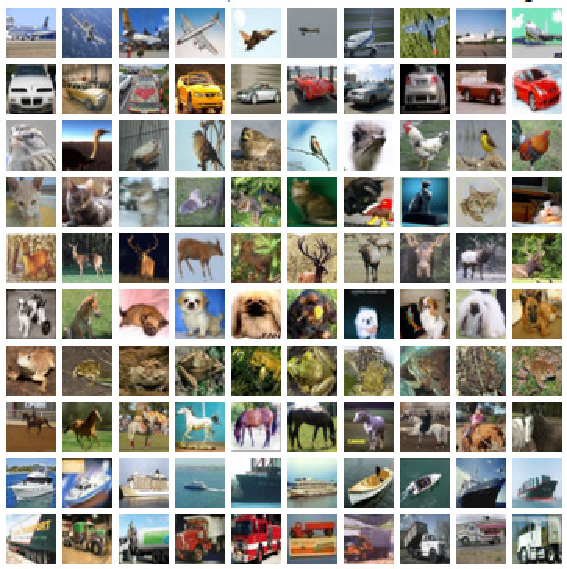
\includegraphics[width=10cm]{man-source/images/ch3/pic3-2.pdf}
		\caption{Фрагмент базы изображений CIFAR-10}				
		\label{fig:cifar_dataset}
	\end{center}
\end{figure}

Выборка CIFAR-100 идентична выборке CIFAR-10 по параметрам изображений, которые в нее включены, но отличается количеством представленных классов изображений (в этой выборке общее количество классов составляет 100). Общая размерность выборки составляет также 60.000 изображений, по 600 изображений на каждый класс.

Выборки CIFAR-10 и CIFAR-100 разделены авторами на обучающую и тестовую подвыборки (объемом 50.000 и 10.000 изображений соответственно).

%Выполнение экспериментов с использованием выборок большого размера занимает достаточно продолжительное время. Эта проблема может быть решена проведением расчетов с использованием видеокарт nVidia, поддерживающих технологию CUDA (например, ускорителей A100 или V100, доступных при использовании сервиса Google Colab \cite{googlecolab}). Существуют другие способы ускорения расчетов, производимых при обучении нейронной сети, например, использование вычислительных кластеров \cite{n16}.

%Количество входов обучаемой НС определялось размерами образов из базы MNIST (784), количество слоев и нейронов в каждом слое выявлялось экспериментальным путем. На каждом слое использовалась сигмоидная функция активации. 

\subsection{Параметры вычислительного эксперимента и результаты}

В качестве целевой модели для решения задачи распознавания изображений из выборки MNIST была выбрана сверточная нейронная сеть с параметрами, представленными в таблице \ref{table:mnist_conv_model}.

\begin{table} [!h]
  \caption{MNIST: основные параметры используемой модели}\label{table:mnist_conv_model}
\centering
\begin{tabular}{| p{7cm} | p{8cm} |}
  \hline
    \textbf{Параметр} & \textbf{Значение}\\
    \hline
    Архитектура & 40Х5Х5 -- 40Х5Х5 -- 640Х320 -- 320Х160 -- 160Х10\\
    \hline
    Функция активации & ReLU \\
    \hline
    Функция активации на последнем слое & Softmax \\
    Начальная инициализация параметров & Нормальное распредение \\
    \hline
\end{tabular}
\end{table}

Первые (сверточные) слои обозначены условно как \textit{K} x \textit{S} x \textit{S}, где \textit{K} обозначает количество ядер свертки в соответствующем слое, a \textit{S} x \textit{S} -- размерность ядра свертки.

Как видно из представленной выше таблицы, использовалась архитектура с 5 обрабатывающими слоями, 2 из которых сверточные, а 3 -- полносвязные. При этом общее число параметров модели составило 299.170.

В качестве функции активации использовалась функция ReLU на всех слоях сети, за исключением последнего слоя, на котором применялась softmax-функция. Использование ReLU позволило варианту обучения без предобучения начать процесс и завершить его с приемлемым значением эффективности.

В таблице \ref{table:mnist_comparing_params} приведены основные используемые параметры обучения. 

\begin{table} [!h]
  \caption{MNIST: основные параметры обучения}\label{table:mnist_comparing_params}
\centering
\begin{tabular}{| p{3cm} | p{6cm} | p{2.5cm} |}
  \hline
    \textbf{Этап} & \textbf{Параметр} & \textbf{Значение}\\
    \hline
    Предобучение & Скорость обучения & 0,000125\\
    \cline{2-3}
    & Размер мини-батча & 128 \\
    \cline{2-3}
    & Моментный параметр & [0,5; 0,9] \\
    \cline{2-3}
    & Количество эпох обучения & 30\\
    \hline
    Обучение & Скорость обучения & 0,001\\
    \cline{2-3}
    & Размер мини-батча & 128 \\
    \cline{2-3}
    & Моментный параметр & 0,9 \\
    \cline{2-3}
    & Количество эпох обучения & 50\\
    \hline
\end{tabular}
\end{table}

Помимо классического и предложенного методов предобучения в ходе проведения экспериментов был протестирован подход, при котором первый слой нейросетевой модели предобучается с использованием классического метода обучения RBM, а все прочие слои, кроме последнего классифицирующего -- с использованием предлагаемого подхода REBA. Будем обозначать такой вариант предобучения как гибридный (HREBA).

Эксперименты проводились с одной и той же начальной инициализацией параметров для всех методов серией в 10 попыток, получаемые результаты затем усреднялись. В ходе эксперимента сравнивались четыре основных варианта обучения: 
\begin{easylistNum}
    & BP -- обучение без предобучения; 
    & REBA -- обучение с предобучением (предлагаемый подход); 
    & HREBA -- обучение с предобучением (гибридный подход);
    & C-RBM -- обучение с классическим методом предобучения).
\end{easylistNum}

В результате были получены показатели эффективности для вышеперечисленных методов, представленные в таблице \ref{table:mnist_results}.

\begin{table} [!h]
  \caption{MNIST: результаты обучения}\label{table:mnist_results}
\centering
\begin{tabular}{| p{6cm} | p{6cm} |}
  \hline
    \textbf{Метод обучения} & \textbf{Эффективность, \%}\\
    \hline
    BP & 99.367\\
    \hline
    REBA & 99.371\\
    \hline
    HREBA & \textbf{99.458}\\
    \hline
    C-RBM & 99.447\\
    \hline
\end{tabular}
\end{table}

Как видно из представленных результатов, лучший средний показатель был достигнут гибридным методом HREBA, сочетающим в себе предобучение классическим и предложенным подходом, при этом максимальная эффективность была получена этим же методом и составила \textbf{99.53} \%.

При проведении экспериментов с выборками CIFAR-10 и CIFAR-100 использовалась модель с архитектурой, представленной в таблице \ref{table:cifar_comparison_params}.

Для выборки CIFAR-100 изменения в архитектуре модели коснулись только последнего слоя (вместо 10 выходных нейронов использовалось 100 -- по количеству классов в данной выборке).

\begin{table}[!h]
    \caption{CIFAR-10/CIFAR-100: основные параметры используемых моделей}\label{table:cifar_comparison_params}
    \begin{tabular}{|p{7cm}|p{8cm}|}
        \hline
        \textbf{Параметр} & \textbf{Значение}\\
        \hline
        Архитектура & 64Х5Х5 -- 32Х5Х5 -- 800Х128 -- 128Х10/100\\
        \hline
        Функция активации & ReLU - Tanh - ReLU \\
        \hline
        Функция активации на последнем слое & Softmax \\
        \hline
        Начальная инициализация параметров & Нормальное распредение \\
        \hline
        Общее число параметров модели & 159.914
        \\
        \hline
    \end{tabular}
\end{table}

В результате были получены показатели эффективности для вышеперечисленных методов, представленные в таблице \ref{table:cifar_10_results} (для выборки CIFAR-10) и \ref{table:cifar_100_results} (для выборки CIFAR-100).

\begin{table} [!h]
  \centering
  \caption{CIFAR-10: результаты обучения}\label{table:cifar_10_results}
  \begin{tabular}{| p{6cm} | p{6cm} |}
    \hline
      \textbf{Метод обучения} & \textbf{Эффективность, \%}\\
      \hline
      BP & 69.74\\
      \hline
      REBA & 71.20\\
      \hline
      HREBA & \textbf{71.59}\\
      \hline
      C-RBM & 71.51\\
      \hline
  \end{tabular}
\end{table}

Лучший результат был получен методом HREBA и составил \textbf{72.32 \%}.

\begin{table} [!h]
  \centering
  \caption{CIFAR-100: результаты обучения}\label{table:cifar_100_results}
  \begin{tabular}{| p{6cm} | p{6cm} |}
    \hline
      \textbf{Метод обучения} & \textbf{Эффективность, \%}\\
      \hline
      BP & 36.83\\
      \hline
      REBA & 38.9\\
      \hline
      HREBA & \textbf{39.86}\\
      \hline
      C-RBM & 39.71\\
      \hline
  \end{tabular}
\end{table}

Лучший результат также был получен методом HREBA и составил \textbf{40.26\%}.

% Мы использовали следующие параметры обучения: скорость обучения -- 0,1 для REBA и 0,2 для классического метода RBM, размер мини-батча -- 100, количество эпох предобучения -- 10, количество эпох <<тонкой>> настройки -- 100. Также мы использовали параметр регуляризации L2, равный 0,00001.

% Результаты экспериментов представлены в таблице \ref{table:tbl2}. \textbf{MSE} определяет ошибку обучения, \textbf{MS} -- ошибку обобщения, \textbf{Ошибка, \%}, \% -- процент ошибочно распознанных изображений, \textbf{К-во эпох} -- число эпох для классического и гибридного метода предобучения.

% \begin{table}[H]
% 	\caption{Сравнение методов предобучения (MNIST)}
% 	\label{table:tbl2}
% 	\centering
% 	\begin{tabularx}{\hsize}{| c | c | c | c | X |}
% 		\hline
% 		\textbf{Метод} & \textbf{MSE} & \textbf{MS} & \textbf{Ошибка, \%} & \textbf{Кол-во эпох}\\
% 		\hline
% 		Classic RBM & 6,178e-6  & 0,0235 & 1,23 & 10 \\
% 		\hline
% 		Hybrid REBA (9+1) & 5,962e-6 & 0,0224 & \textbf{1,09} & 9+1 \\										
% 		\hline
% 	\end{tabularx}			
% \end{table}	

% Необходимо отметить, что нейронная сеть обученная на полной выборке из базы MNIST, ошибается на образах, многие из которых трудноразличимы даже для человеческого глаза (рис. \ref{fig:incorrect_recognized_samples})

% \begin{figure}[h]
% 	\begin{center}
% 		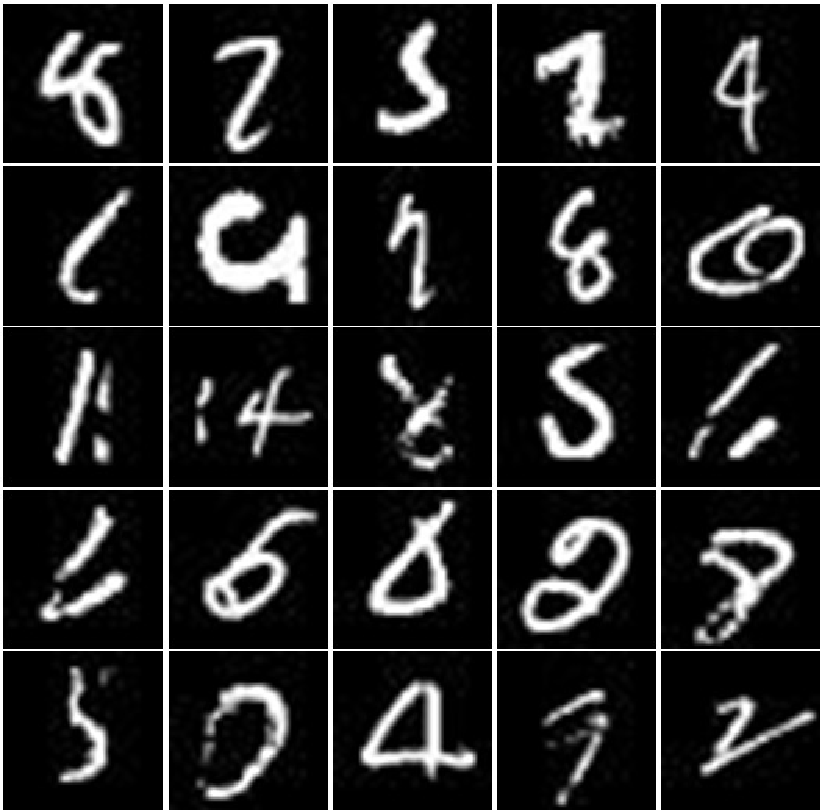
\includegraphics[width=8cm]{man-source/images/ch3/pic3-12.pdf}
% 		\caption{Образы, некорректно распознанные НС}		
% 		\label{fig:incorrect_recognized_samples}
% 	\end{center}
% \end{figure}

% \section{Визуализация данных}

% Для иллюстрации производительности метода REBA мы провели эксперименты по визуализации данных выборки MNIST. Для отображение 784-мерных данных, соответствующих количеству пикселей в исходном выражении нами использовался глубокая автоассоциативная сеть с архитектурой 784-500-500-250-10-2. Для всех слоев, за исключением среднего слоя, использовалась сигмоидная функция активации. На среднем слое применялась линейная функция. 

% Вначале выполнялось предобучение в соответствии с <<жадным>> послойным алгоритмом. Затем выполнялось <<разворачивание>> сети в полную архитектуру и производилась <<тонкая>> настройка параметров. Для предобучения использовались следующие параметры: скорость обучения -- 0.2 (REBA), скорость обучения для среднего слоя -- 0.001.

% Визуализация для первых 5000 образов из тестовой выборки представлена на рис. \ref{fig:mnist_dataset_visualize}

% \begin{figure}[ht]
% 	\centering
% 	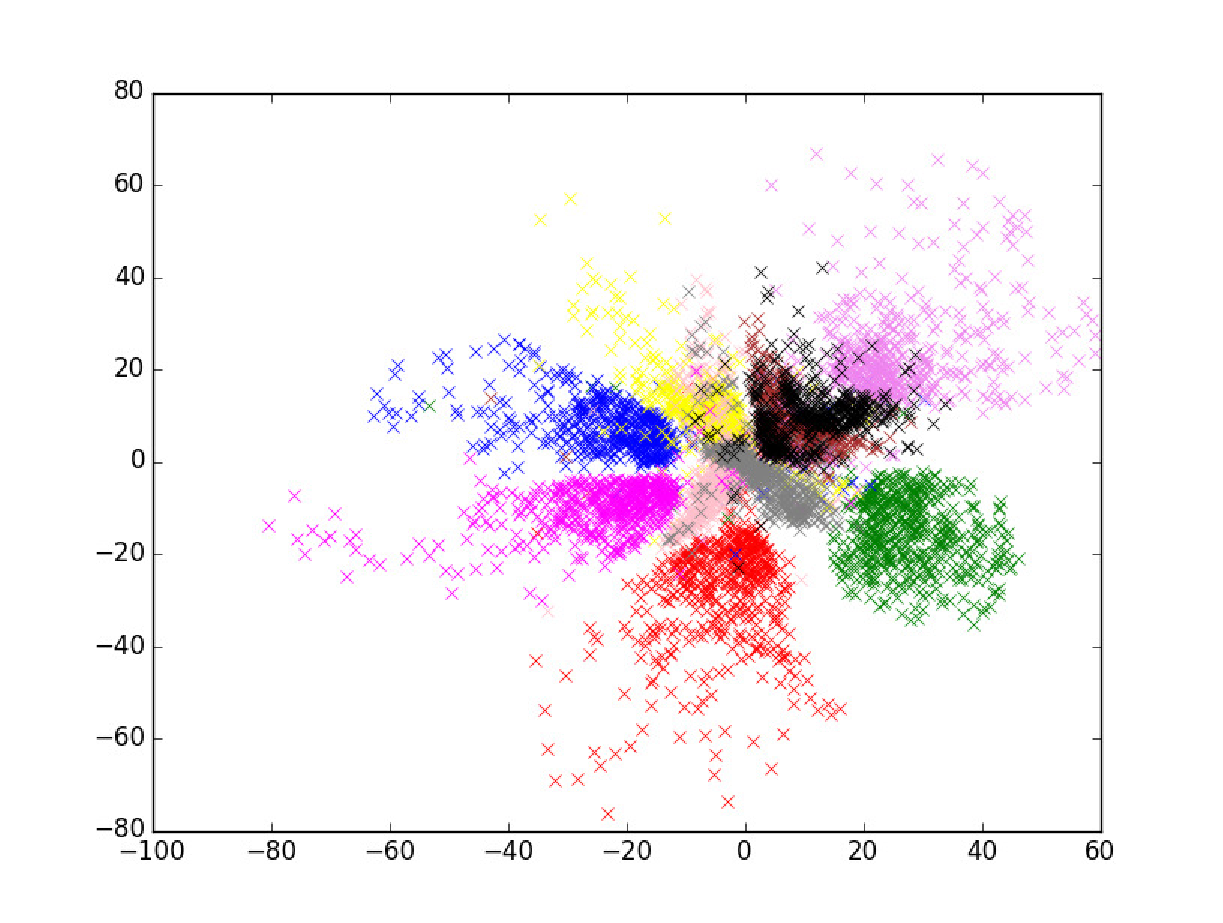
\includegraphics[width=16cm]{man-source/images/ch3/pic3-1.pdf}
% 	\caption{Визуализация рукописных цифр из базы MNIST}
% 	\label{fig:mnist_dataset_visualize}
% \end{figure}

% На рисунке видно, что в процессе обучения выделились кластеры в 2-ном пространстве главных компонент, соответствующие каждой цифре из оригинальной выборки. Таким образом, сеть не располагая информацией о каких-либо метках для исходных данных, смогла выделить области наибольшего подобия.

% \section{Семантическое кодирование}

% \subsection{Постановка задачи}
% В качестве обучающей выборки для решения задачи построения бинарных семантических кодов изображений нами была использована база CIFAR-10.  Данная выборка предоставляет богатый материал для выявления семантических особенностей \cite{n17}. Она включает в себя 50.000 изображений технических средств и живых существ, принадлежащий 10 различным классам (рис. \ref{fig:cifar_dataset}). Каждое изображение имеет размер 32Х32 пикселя.

% Помимо этого, CIFAR-10 включает тестирующую выборку, состоящую из 10.000 изображений.

% \begin{figure}[h]
% 	\begin{center}
% 		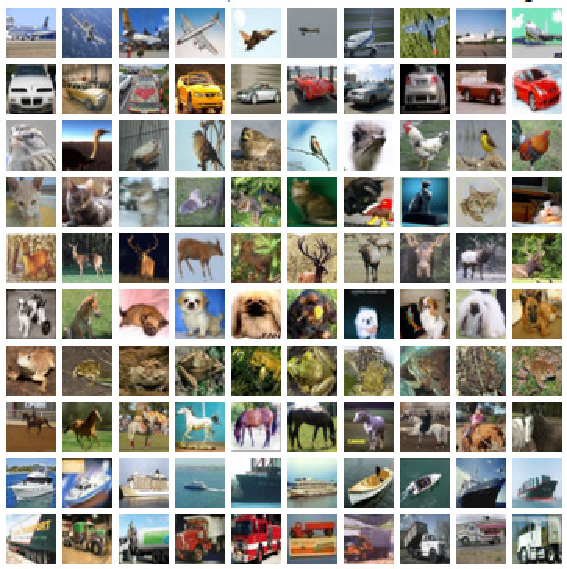
\includegraphics[width=12cm]{man-source/images/ch3/pic3-2.pdf}
% 		\caption{Фрагмент базы изображений CIFAR-10}				
% 		\label{fig:cifar_dataset}
% 	\end{center}
% \end{figure}

% Семантическое кодирование (хеширование) относится к более сложному и не менее важному типу задач, решение которого позволяет сформировать бинарный код ограниченной длины, емко и однозначно описывающий изображение в редуцированном признаковом пространстве. С помощью такого преобразования можно сформировать базу изображений, представленных лишь бинарным кодом. На основе такой базы можно построить систему релевантного поиска изображений.

% \subsection{Структура сети и основные параметры обучения}
% Для решения задачи нами использовалась 11-слойная ассоциативная нейронная сеть с архитектурой 3072-4096-2048-1024-512-256-512-1024-2048-4096-3072. На среднем слое такой сети формируется вектор вещественных значений из отрезка [0, 1], элементы которого затем округляются. Таким образом формируется бинарный код изображения. Легко видеть, что таким образом может быть закодировано $2^{256}$ изображений, что более чем достаточно для базы CIFAR-10. Нами использовались все изображения из обучающей выборки указанной базы.

% Обучение проводилось в два этапа. На первом этапе предобучались соответствующие RBM, формирующие кодирующие слои сети. Исходные данные перед обучением были стандартизованы: из каждого компонента вектора изображения вычиталось его среднее значение по всем изображениям выборки и затем полученное значение делилось на стандартное отклонение по всем компонентам всех изображений. Данное преобразование определило тип первой обучаемой машины Больцмана -- линейно-бинарная RBM \cite{n4}. Остальные машины обучались как бинарные RBM.

% Каждая RBM обучалась на протяжении 100 эпох мини-батчами по 100 элементов. Для линейно-бинарной RBM использовалось скорость обучения 0,001, для бинарной -- 0,01. Помимо этого для ускорения процесса обучения использовался моментный параметр, равный 0,9.

% После проведения предобучения выполнялось обучение развернутой автоассоциативной сети методом обратного распространения ошибки. Параметры обучения: скорость -- $1e^{-6}$, количество эпох обучения -- 150, моментный параметр -- 0.9.

% После выполнения обучения, результат оценивался вычислением расстояния Хэмминга между бинарными кодами для тестового изображения и изображениями из базы (формула \ref{chemming_dist}) После этого полученный ряд значений сортировался по возрастанию для выделения наиболее релевантных результатов.

% \begin{equation}
% 	\label{chemming_dist}
% 	H(v_1,v_2) = \sum_{i=1}^{n}|v_1^i-v_2^i|
% \end{equation}

% Вычисления, производимые в процессе обучения глубокой автоассоциативной нейронной сети производились на видеокарте GTX 750 Ti и заняли приблизительно 90 минут.

% Программный код на языке программирования Python для выполнения предобучения данной сети приведен в приложении 1.

% \subsection{Результаты обучения}
% Мы протестировали нашу модель двумя способами. Первый вариант предусматривал визуальное сравнение оригинального и восстановленного изображения. Некоторые из выполненных тестов представлены на рисунке \ref{fig:restore_images_results}.

% \begin{figure}[h]
% 	\begin{center}
% 		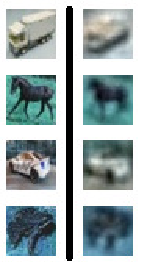
\includegraphics[width=40mm]{man-source/images/ch3/pic3-3.pdf}
% 		\caption{Оригинальные и восстановленные нейронной сетью изображения}				
% 		\label{fig:restore_images_results}
% 	\end{center}
% \end{figure}

% Второй вариант тестирования заключался в подаче на обученную автоассоциативную сеть изображения, получения его бинарного кода с промежуточного слоя сети и вычисления расстояния Хэмминга для всех остальных изображений. Отсортировав получившуюся последовательность по возрастанию, можно изучить наиболее релевантные результаты поиска (рис. \ref{fig:search_template}).

% \begin{figure}[h]
% 	\begin{center}
% 		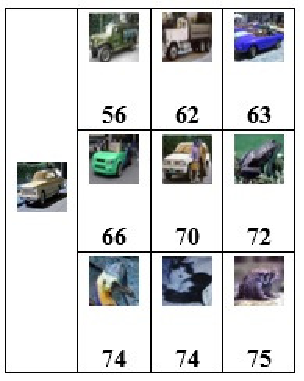
\includegraphics[width=8cm]{man-source/images/ch3/pic3-4.pdf}
% 		\caption{Поисковый шаблон и результаты поиска}				
% 		\label{fig:search_template}
% 	\end{center}
% \end{figure}

% Исходя из представленных данных, можно отметить, что с увеличением расстояния Хэмминга количество изображений того же класса, что и целевое изображение постепенно уменьшается.

\section{Редуцирование параметров НС}

Продемонстрируем эффективность предложенного подхода на примере редуцирования различных архитектур полносвязных нейронных сетей, применяемых для классификации изображений из выборок MNIST \cite{mnist}, CIFAR10 и CIFAR100 \cite{krizhevsky2009learning}.
Были проведены серии экспериментов, включающих различные используемые выборки, архитектуры и варианты предобучения. В рамках одной выборки и архитектуры НС текущая инициализация параметров сохранялась для возможности сравнения эффективности различных вариантов предобучающей процедуры.
Ниже для рассматриваемых выборок приведены основные параметры, включающие скорость обучения, размер мини-батча, моментный параметр и количество эпох для предобучения и <<тонкой настройки>> моделей (табл. \ref{table:reduce_training_params}).

\begin{table} [!h]
  \small
  \caption{Основные параметры обучения}\label{table:reduce_training_params}
\centering
\begin{tabular}{| p{3cm} | p{6cm} | p{2cm} |}
  \hline
    \textbf{Этап} & \textbf{Параметр} & \textbf{Значение}\\
    \hline
    Обучение & Скорость обучения & 0.05-0.1\\
    \cline{2-3}
    & Размер мини-батча & 100 \\
    \cline{2-3}
    & Моментный параметр & 0.9 \\
    \cline{2-3}
    & Количество эпох обучения & 50-100\\
    \hline
    Предобучение & Скорость обучения & 0.05-0.2\\
    \cline{2-3}
    & Размер мини-батча & 32-100 \\
    \cline{2-3}
    & Моментный параметр & [0.5, 0.9] \\
    \cline{2-3}
    & Количество эпох обучения & 10\\
    \hline
\end{tabular}
\end{table}

В результате вычислительного эксперимента были получены результаты для различных выборок, архитектур НС и значений параметра редуцирования t (табл. \ref{table:mnist_1}-\ref{table:cifar_100}).

\begin{table} [!h]
  \small
  \caption{784-800-800-10, MNIST}\label{table:mnist_1}
\centering
\begin{tabular}{| p{2cm} | p{4cm} | p{4cm} | p{4cm} |}
  \hline
    \textbf{Тип} & \textbf{Эффективность, \%, C-RBM / REBA} & \textbf{Количество параметров, C-RBM / REBA} & \textbf{Редуцировано параметров, \%, C-RBM / REBA}\\
    \hline
    без редуц. & \textbf{98.63} / 98.33 & 1276810 / 1276810 & 0/0\\
    \hline
    t=0.2 & \textbf{98.61} / 98.27 & \textbf{233760} / 279635 & \textbf{81.69} / 78.1\\
    \hline
    t=0.5 & 98.03 / \textbf{98.05} & \textbf{32524} / 32817 & \textbf{97.45} / 97.43\\
    \hline
    t=0.8 & \textbf{97.1} / 96.48 & 17061 / \textbf{12217} & 98.66 / \textbf{99.04}\\
    \hline
\end{tabular}
\end{table}

\begin{table} [!h]
  \small
  \caption{784-1600-1600-800-800-10,  MNIST}\label{table:mnist_2}
\centering
\begin{tabular}{| p{2cm} | p{4cm} | p{4cm} | p{4cm} |}
  \hline
    \textbf{Тип} & \textbf{Эффективность, \%, C-RBM / REBA} & \textbf{Количество параметров, C-RBM / REBA} & \textbf{Редуцировано параметров, \%, C-RBM / REBA}\\
    \hline
    wr & \textbf{98.76} / 98.37 & 5747210 / 5747210 & 0/0\\
    \hline
    t=0.2 & 98.51 / \textbf{98.55} & \textbf{710734} / 781103 & \textbf{87.63} / 86.41\\
    \hline
    t=0.5 & 98.01 / \textbf{98.03} & 54709 / \textbf{43867} & 99.05 / \textbf{99.24}\\
    \hline
    t=0.8 & \textbf{96.9} / 93.08 & 25385 / \textbf{14914} & 99.56 / \textbf{99.74}\\
    \hline
\end{tabular}
\end{table}

\begin{table} [!h]
  \small
  \caption{3072-1024-512-256-128-64-10, CIFAR10}\label{table:cifar_10_1}
\centering
\begin{tabular}{| p{2cm} | p{4cm} | p{4cm} | p{4cm} |}
  \hline
    \textbf{Тип} & \textbf{Эффективность, \%, C-RBM / REBA} & \textbf{Количество параметров, C-RBM / REBA} & \textbf{Редуцировано параметров, \%, C-RBM / REBA}\\
    \hline
    wr & \textbf{58.56} / 55.85 & 3844682 / 3844682 & 0/0\\
    \hline
    t=0.2 & \textbf{58.69} / 54.37 & 409211 / \textbf{227072} & 89.36 / \textbf{94.09}\\
    \hline
    t=0.5 & \textbf{42.08} / 41.2 & 29033 / \textbf{11320} & 99.24 / \textbf{99.71}\\
    \hline
    t=0.8 & \textbf{23.02} / 10.0 & 10058 / \textbf{4886} & 99.74 / \textbf{99.87}\\
    \hline
\end{tabular}
\end{table}

\begin{table} [!h]
  \small
  \caption{3072-512-256-128-64-10, CIFAR10 }\label{table:cifar_10_2}
\centering
\begin{tabular}{| p{2cm} | p{4cm} | p{4cm} | p{4cm} |}
  \hline
    \textbf{Тип} & \textbf{Эффективность, \%, C-RBM / REBA} & \textbf{Количество параметров, C-RBM / REBA} & \textbf{Редуцировано параметров, \%, C-RBM / REBA}\\
    \hline
    wr & \textbf{57.28} / 53.69 & 1746506 / 1746506 & 0/0\\
    \hline
    t=0.2 & \textbf{56.83} / 41.72 & 220037 / \textbf{126846} & 87.40 / \textbf{92.73}\\
    \hline
    t=0.5 & \textbf{45.29} / 44.93 & 20431 / \textbf{11383} & 98.83 / \textbf{99.35}\\
    \hline
    t=0.8 & 10.0 / 10.0 & 8599 / 3797 & 99.51 / 99.78\\
    \hline
\end{tabular}
\end{table}

\begin{table} [!h]
  \small
  \caption{3072-3072-1024-512-256-128-64-100, CIFAR100}\label{table:cifar_100}
\centering
\begin{tabular}{| p{2cm} | p{4cm} | p{4cm} | p{4cm} |}
  \hline
    \textbf{Тип} & \textbf{Эффективность, \%, C-RBM / REBA} & \textbf{Количество параметров, C-RBM / REBA} & \textbf{Редуцировано параметров, \%, C-RBM / REBA}\\
    \hline
    wr & 20.84 / \textbf{21.63} & 13290788 / 13290788 & 0/0\\
    \hline
    t=0.2 & 20.77 / \textbf{21.01} & 1304525 / \textbf{703319} & 90.18 / \textbf{94.71}\\
    \hline
    t=0.5 & \textbf{13.4} / 1.0 & 49847 / \textbf{24636} & 99.62 / \textbf{99.81}\\
    \hline
    t=0.8 & \textbf{2.67} / 1.0 & 21329 / \textbf{16977} & 99.84 / \textbf{99.87}\\
    \hline
\end{tabular}
\end{table}
% \begin{figure}[h]
% 	\begin{center}
% 		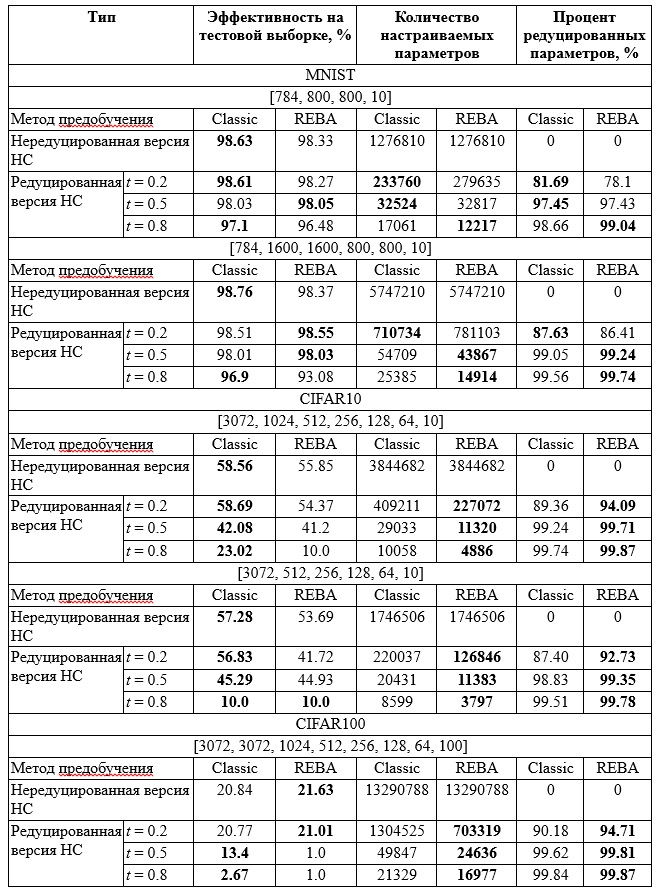
\includegraphics[width=18cm]{man-source/images/ch3/pic3-13.jpg}
% 		\caption{Результаты редуцирования}				
% 		\label{fig:reduce_results}
% 	\end{center}
% \end{figure}

Как видно из приведенных результатов, исследуемые архитектуры в целом сохраняют обобщающую способность, будучи редуцированными более чем на 80 процентов.

Также можно заметить, что чем больше настраиваемых параметров в модели, тем эффективней осуществляется редуцирование. Однако с увеличением параметра редуцирования эффективность исходной сети постепенно снижается, так как редуцированию начинают подвергаться параметры, наличие которых влияет на выходы нейронной сети.

Полученные результаты обосновывают возможность предобучения глубокой нейронной сети с использованием неконтролируемой процедуры без получения эффекта переобучения и снижения эффективности модели, так как в процессе предобучения фактически снижается влияние определенных параметров модели на итоговую выходную активность сети. Такие параметры имеют ``паразитический'' характер и фактически являются фактором переобучения модели. На этапе <<тонкой настройки>> модели они не модифицируются и могут быть удалены после этапа предобучения.
% Продемонстрируем эффективность предложенного подхода на примере редуцирования различных архитектур полносвязных нейронных сетей, применяемых для классификации изображений из выборок MNIST [12], CIFAR10 и CIFAR100 [13]. Данные выборки являются классическими для проверки эффективности моделей машинного обучения.
% Нами были проведены серии экспериментов, включающих различные используемые выборки, архитектуры и варианты предобучения. В рамках одной выборки и архитектуры НС текущая инициализация параметров сохранялась для возможности сравнения эффективности различных вариантов предобучающей процедуры.
% Ниже для рассматриваемых выборок приведены основные параметры, включающие скорость обучения, размер мини-батча, моментный параметр и количество эпох для предобучения и дообучения моделей (табл \ref{table:reduce_training_params}).

% \begin{table} [H]
%   \small
%   \caption{Основные параметры обучения}\label{table:reduce_training_params}
% \begin{tabularx}{\hsize}{| X | X | X |}
%   \hline
%     \multicolumn{2}{|c|}{\textbf{Функции активации}} &
%     \textbf{Сигмодные на все слоях, кроме последнего (линейная)}\\
%     \hline
%     \multirow{4}{*}{Обучение} & Скорость обучения & 0.05-0.1\\
%     \cline{2-3}
%     & Размер мини-батча & 100 \\
%     \cline{2-3}
%     & Моментный параметр & 0.9 \\
%     \cline{2-3}
%     & Количество эпох обучения & 50-100\\
%     \hline
%     \multirow{4}{*}{Предобучение} & Скорость обучения & 0.05-0.2\\
%     \cline{2-3}
%     & Размер мини-батча & 32-100 \\
%     \cline{2-3}
%     & Моментный параметр & [0.5, 0.9] \\
%     \cline{2-3}
%     & Количество эпох обучения & 10\\
%     \hline
% \end{tabularx}
% \end{table}

% В результате вычислительного эксперимента были получены результаты для различных архитектур НС и значений параметра редуцирования t (табл. \ref{fig:reduce_results}).

% \begin{figure}[h]
% 	\begin{center}
% 		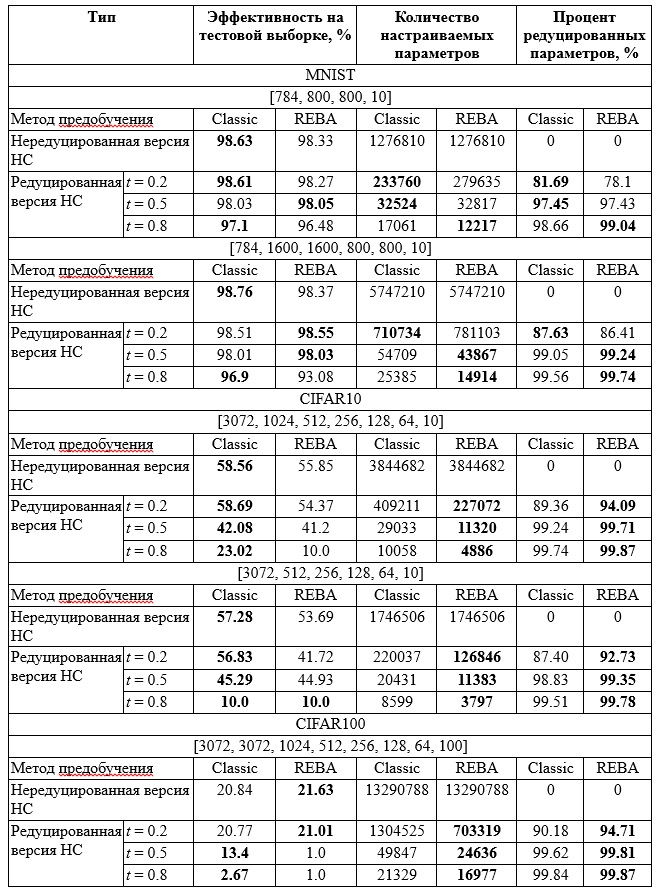
\includegraphics[width=18cm]{man-source/images/ch3/pic3-13.jpg}
% 		\caption{Результаты редуцирования}				
% 		\label{fig:reduce_results}
% 	\end{center}
% \end{figure}
% \begin{table} [H]
%   \small
%   \caption{Результаты редуцирования}\label{table:reduce_results}
% \begin{tabularx}{\hsize}{| X | X | X | X | X | X | X | X |}
%   \hline
%     \multicolumn{2}{|c|}{\textbf{Тип}} & &
%     \multicolumn{2}{|c|}{\textbf{Эффективность на тестовой выборке, \%}} & & \multicolumn{2}{|c|}{\textbf{Количество настраиваемых параметров}} & & \multicolumn{2}{|c|}{\textbf{Процент редуцированных параметров, \%}} &\\
%     \hline
%     \multicolumn{8}{|c|}{MNIST}\\
%     \hline
%     \multicolumn{8}{|c|}{[784, 800, 800, 10]}\\
%     \hline
%     \multicolumn{2}{|c|}{\textbf{Метод предобучения}} & Classic & REBA & Classic & REBA & Classic & REBA\\
%     % \cline{2-3}
%     % & Размер мини-батча & 100 \\
%     % \cline{2-3}
%     % & Моментный параметр & 0.9 \\
%     % \cline{2-3}
%     % & Количество эпох обучения & 50-100\\
%     % \hline
%     % \multirow{4}{}{Предобучение} & Скорость обучения & 0.05-0.2\\
%     % \cline{2-3}
%     % & Размер мини-батча & 32-100 \\
%     % \cline{2-3}
%     % & Моментный параметр & [0.5, 0.9] \\
%     % \cline{2-3}
%     % & Количество эпох обучения & 10\\
%     \hline
% \end{tabularx}
% \end{table}

Помимо редуцирования параметров, было выполнено так называемое архитектурное редуцирование (шаг 3 алгоритма), на котором производилось упрощение структуры слоев моделей за счет исключения нейронов с нулевыми векторами связей.

В следующих таблицах (\ref{table:architect_reduce_mnist_one}, \ref{table:architect_reduce_mnist_two}) приведены результаты архитектурного редуцирования для двух различных архитектур и обучающей выборки MNIST. Для предобучения использовался метод REBA.

\begin{table} [!h]
  \small
  \caption{784-800-800-10, MNIST}\label{table:architect_reduce_mnist_one}
    \centering
    \begin{tabular}{| p{2cm} | p{6cm} | p{6cm} |}
    \hline
        \textbf{Параметр} & \textbf{Исходная} & \textbf{Редуцированная}\\
    \hline
    t=0.2 & 784-800-800-10 & 784-800-556-10\\
    \hline
    t=0.5 & -//- & 784-710-422-10\\
    \hline
    t=0.9 & -//- & 784-91-114-10\\
    \hline
    \end{tabular}
    \end{table}
    
\begin{table} [!h]
  \small
    \caption{784-1600-1600-800-800-10, MNIST}\label{table:architect_reduce_mnist_two}
    \centering
    \begin{tabular}{| p{2cm} | p{6cm} | p{6cm} |}
    \hline
        \textbf{Параметр} & \textbf{Исходная} & \textbf{Редуцированная}\\
    \hline
    t=0.2 & 784-1600-1600-800-800-10 & 784-889-192-686-221-10\\
    \hline
    t=0.5 & -//- & 784-464-157-567-182-10\\
    \hline
    t=0.9 & -//- & 784-17-101-118-50-10\\
    \hline
    \end{tabular}
    \end{table}
    
Из приведенных таблиц можно заметить, что для моделей с большим количеством слоев и нейронов в каждом слое вероятность архитектурного редуцирования выше и оно начинает происходить уже для сравнительно небольших значений параметра редуцирования \textit{t}, в том время как для более <<поверхностных>> моделей оно существеннее проявляется только для больших значений параметра. Стоит отметить, что архитектуры, которые сохраняют почти все нейроны (например, \ref{table:architect_reduce_mnist_one}, архитектура при \textit{t}=0.2), все же при этом теряют для каждого нейрона основную часть связей (сохранение нейрона в данном случае будет иметь место, даже при сохранении одной связи нейрона с предыдущим слоем).

\section{Выводы}

\begin{easylistNum}
    & Проведен сравнительный анализ методов предобучения ГНС для задачи сжатия данных с использованием автоэнкодерной модели НС.
    & Проведен сравнительный анализ методов предобучения ГНС для задачи распознавания образов с использованием выборок MNIST, CIFAR-10 и CIFAR-100. Предложена модификация метода предобучения.
    %& Проведена серия экспериментов по визуализации данных выборки MNIST с применением предлагаемого метода предобучения.
    %& Проведены экспериментальные исследования по решению задачи семантического кодирования изображений из выборки CIFAR-10 с применением глубокой автоассоциативной нейронной сети и предлагаемого метода предобучения.
    & Проведены экспериментальные исследования редуцирования параметров глубокой нейронной сети с использованием различных методов предобучения и архитектур ГНС.
\end{easylistNum}

% \chapter{МЕТОДИКА И СРЕДСТВА АВТОМАТИЗАЦИИ ПРОЦЕССА ПОСТРОЕНИЯ И МОДИФИКАЦИИ РЕШАТЕЛЕЙ ЗАДАЧ}
% %\addcontentsline{toc}{chapter}{МЕТОДИКА И СРЕДСТВА АВТОМАТИЗАЦИИ\\ ПРОЦЕССА ПОСТРОЕНИЯ И МОДИФИКАЦИИ РЕШАТЕЛЕЙ ЗАДАЧ}	

% Как уже было сказано выше, все платформенно-независимые компоненты гибридного решателя задач ostis-системы могут быть представлены при помощи SC-кода. При этом речь идет как о спецификациях sc-агентов, так и о полных текстах scp-программ, описывающих алгоритмы работы указанных агентов.

% Таким образом, построение объединенного решателя задач некоторой ostis-системы сводится к разработке особого рода фрагмента базы знаний такой системы. В связи с этим, при построения и модификации решателей могут использоваться все существующие средства автоматизации процесса построения и модификации баз знаний по Технологии OSTIS, рассмотренные, в частности, в работах \cite{Davydenko2016b,Davydenko2017}.

% В рамках данной главы диссертационной работы рассмотрены некоторые аспекты разработки, специфичные конкретно для гибридных решателей задач, в частности, методика построения и модификации таких решателей и средства автоматизации и информационной поддержки процесса построения и модификации решателей, построенных в соответствии с предложенной выше моделью. 

% Как было сказано в главе 1, указанные средства включают систему автоматизации процесса построения и модификации решателей и подсистему информационного обслуживания разработчиков решателей в рамках метасистемы IMS.

% Важнейшим фрагментом метасистемы IMS является библиотека многократно используемых компонентов ostis-систем, в рамках которой выделяется библиотека многократно используемых компонентов решателей задач, построенная с учетом классификации sc-агентов и решателей, представленной в главе 2. Указанная библиотека включает как сами компоненты, так и набор агентов автоматизации поиска нужных компонентов на основе некоторой спецификации.

% Более подробно набор разделов базы знаний IMS, обеспечивающих информационную поддержку разработчиков гибридных решателей задач, рассмотрен в разделе \ref{section_contrib} данной диссертационной работы. В текущей главе основное внимание будет уделено методике построения и модификации решателей задач и системе автоматизации процесса построения и модификации решателей задач, а также библиотеке многократно используемых компонентов решателей задач. 

% Как показано на рисунке~\ref{fig:pic3_1}, разработка методики построения и модификации гибридных решателей задач предполагает разработку формальной онтологии деятельности разработчиков таких решателей; разработка библиотеки многократно используемых компонентов предполагает разработку семантической модели библиотеки, уточняющей виды компонентов и средства их спецификации, а также разработку средств поиска нужного компонента по некоторой заданной спецификации; наконец, система автоматизации процесса построения и модификации решателей задач условно делится на две подсистемы, о чем подробнее будет сказано ниже. Информационная поддержка и консультационное обслуживание разработчиков обеспечивается развитием базы знаний метасистемы IMS, в рамках которой представлены все результаты данной диссертационной работы.

% \begin{figure}[H]
%     \centering
%     \includegraphics[width=\textwidth]{man-source/images/ch3/pic3_1.pdf}
%     \caption{Структура главы 3}
%     \label{fig:pic3_1}
% \end{figure}

% \newpage
% \section{Методика построения и модификации гибридных решателей задач} \label{section_method_1}

% Предлагаемая методика построения и модификации гибридных решателей задач включает несколько этапов. На рисунке~\ref{fig:pic3_2} представлен перечень таких этапов с указанием последовательности их выполнения. Темным фоном отмечены те этапы, которые частично автоматизированы в рамках средств, рассмотренных ниже в данной главе.

% \begin{figure}[H]
%     \centering
%     \includegraphics[width=\textwidth]{man-source/images/ch3/pic3_2.png}
%     \caption{Этапы процесса построения и модификации гибридных решателей задач}
%     \label{fig:pic3_2}
% \end{figure}

% Рассматриваемая методика может быть применена как при разработке объединенных решателей, так и при разработке решателей частного вида, поскольку с формальной точки зрения все они трактуются как неатомарный абстрактный sc-агент. 

% Рассмотрим подробнее каждый из этапов на примере разработки решателя задач интеллектуальной справочной системы (ИСС) по геометрии Евклида, который будет подробнее описан в главе 4.

% \textbf{\textit{Этап1. Формирование требований и спецификация  решателя задач}}

% На данном этапе необходимо четко выделить задачи, решение которых должен обеспечивать решатель задач, продумать предполагаемые способы их решения и на основе данного анализа определить место будущего решателя в общей иерархии решателей, рассмотренной выше. Важность данного этапа заключается с в том, что при правильной классификации существует вероятность того, что в составе библиотеки компонентов уже есть реализованный вариант требуемого решателя. В противном случае, тем не менее, у разработчика появляется возможность включить разработанный решатель в библиотеку компонентов для последующего использования. Данные факты обусловлены тем, что структура библиотеки компонентов решателей задач основана на семантической классификации таких решателей и, соответственно, их компонентов.

% При недостаточно четкой спецификации и классификации разрабатываемого решателя повышается вероятность того, что подходящий решатель не будет найден в библиотеке компонентов даже в случае, если он там есть, а вновь разработанный решатель не сможет быть включен в библиотеку. Таким образом, идея многократного использования уже разработанных компонентов будет нарушена, что существенно повысит затраты на разработку такого решателя. 

% Для первой версии разрабатываемого решателя по геометрии можно выделить такие классы задач, как:

% \begin{easylistNum}
%  & базовый поиск по базе знаний (поиск элементов заданного множества; поиск классов, которым принадлежит заданная сущность; поиск идентификаторов для заданной сущности; поиск декомпозиции заданной сущности; поиск семантической окрестности заданной сущности; поиск всех сущностей, являющихся частными/общими для заданной сущности);
%  & поиск по базе знаний, актуальный для интеллектуальных справочных систем (поиск иллюстраций для заданной сущности; поиск аксиом/теорем заданной формальной теории; поиск понятий, на основе которых определяется заданное понятие; поиск понятий, которые определяются на основе заданного понятия; поиск доказательства заданного логического утверждения, заранее представленного в базе знаний; поиск решения заданной задачи, заранее представленной в базе знаний и др.);
%  & поиск значения заданной величины с использованием простых механизмов логического вывода и стратегии поиска в глубину;
% \end{easylistNum}

% \textbf{\textit{Этап2. Формирование коллектива sc-агентов, входящих в состав разрабатываемого решателя}}

% В случае, когда найти в библиотеке готовый решатель, удовлетворяющий всем предъявляемым требованиям, не представляется возможным, необходимо выделить и специфицировать все компоненты такого решателя.

% Результатом данного этапа является перечень полностью специфицированных \textit{sc-агентов}, которые войдут в состав разрабатываемого решателя, с их иерархией вплоть до \textit{атомарных sc-агентов}. В рамках данного этапа очень важно проектировать коллектив агентов таким образом, чтобы максимально задействовать уже имеющиеся в библиотеке многократно используемые компоненты, а при отсутствии нужного компонента – иметь возможность включить его в библиотеку после реализации. В качестве таких компонентов, в зависимости от сложности разрабатываемого решателя, могут выступать как \textit{атомарные sc-агенты}, так и целые коллективы sc-агентов (\textit{неатомарные \mbox{sc-агенты}}).

% При разработке перечня агентов (в том числе их спецификаций) необходимо соблюдать ряд принципов:

% \begin{easylist}
% &	каждый разрабатываемый sc-агент должен быть по возможности предметно независим, т. е. во множество ключевых узлов данного sc-агента не должны входить понятия, имеющие отношение непосредственно к рассматриваемой предметной области. Исключение составляют понятия из общих предметных областей, которые носят междисциплинарный характер (например, отношение \textit{включение*} или понятие \textit{действие}). Данное правило также может быть нарушено в случае, если sc-агент является вспомогательным и ориентирован на обработку какого-либо конкретного класса объектов (например, sc-агенты, выполняющие арифметические вычисления, могут напрямую работать с конкретными отношениями \textit{сложение*} и \textit{умножение*} и т. п.). Всю необходимую для решения задачи информацию sc-агент должен извлекать из семантической окрестности соответствующего инициированного действия. Очевидно, что sc-агент, разработанный с учетом указанных требований, может быть использован при проектировании большего числа ostis-систем, чем в случае, если бы он был реализован с ориентацией на конкретную частную предметную область. После завершения разработки и отладки такой sc-агент должен быть включен в \textit{Библиотеку многократно используемых абстрактных sc-агентов};

% &	не стоит путать понятия sc-агент и агентная программа (в том числе агентная scp-программа). Взаимодействие sc-агентов осуществляется исключительно посредством спецификации информационных процессов в общей памяти, каждый sc-агент реагирует на некоторый класс событий в sc-памяти. Таким образом, каждому sc-агенту соответствует некоторое условие инициирования и одна агентная программа, которая запускается автоматически при возникновении в sc-памяти соответствующего условия инициирования. При этом в рамках данной программы могут сколько угодно раз вызываться различные подпрограммы. Однако не стоит путать инициирование sc-агента, которое осуществляется при появлении в sc-памяти соответствующей конструкции, и вызов подпрограммы другой программой, который предполагает явное указание вызываемой подпрограммы и перечня ее параметров;

% &	каждый sc-агент должен самостоятельно проверять полноту соответствия своего условия инициирования текущему состоянию sc-памяти. В процессе решения какой-либо задачи может возникнуть ситуация, когда на появление одной и той же структуры среагировали несколько sc-агентов. В таком случае выполнение продолжают только те из них, условие инициирования которых полностью соответствует сложившейся ситуации. Остальные sc-агенты в данном случае прекращают выполнение и возвращаются в режим ожидания. Выполнение данного принципа достигается за счет тщательного уточнения спецификаций разрабатываемых sc-агентов. В общем случае условия инициирования у нескольких sc-агентов могут совпадать, например, в случае, когда одна и та же задача может быть решена разными способами и заранее неизвестно, какой из них приведет к желаемому результату;

% &	необходимо помнить, что неатомарный sc-агент с точки зрения других sc-агентов, не входящих в его состав, должен функционировать как целостный sc-агент (выполнять логически атомарные действия), что накладывает определенные требования на спецификации атомарных sc-агентов, входящих в его состав: как минимум, необходимо, чтобы в составе неатомарного sc-агента присутствовал хотя бы один атомарный sc-агент, условие инициирования которого полностью совпадает с условием инициирования данного неатомарного sc-агента;

% &	при необходимости реализации нового sc-агента следует руководствоваться следующими принципами выделения атомарных абстрактных \mbox{sc-агентов}:

% \begin{easylistNum}

% & проектируемый sc-агент должен быть максимально независим от предметной области, что позволит в дальшейшем использовать его при разработке решателей максимально возможного числа ostis-систем. При этом универсальность предполагает не только минимизацию числа ключевых узлов sc-агента, но и выделение класса действий, выполняемых данным sc-агентом таким образом, чтобы имело смысл включить данный sc-агент в \textit{Библиотеку многократно используемых абстрактных sc-агентов} и использовать его при разработке решателей других ostis-систем. Не следует искусственно увязывать ряд действий в один sc-агент и, наоборот, расчленять одно самодостаточное действие на поддействия: это вызовет сложности восприятия принципов работы sc-агента разработчиками и не позволит использовать sc-агент в ряде систем (например, в обучающих системах, которые должны объяснять ход решения пользователю);

% & акт деятельности каждого sc-агента (выполняемое данным sc-агентом действие) должен быть логически целостным и завершенным. Следует помнить, что все sc-агенты взаимодействуют исключительно через общую память и избегать ситуаций, в которых инициирование одного sc-агента осуществляется путем явной генерации известного условия инициирования другим \mbox{sc-агентом} (т. е., по сути, явным непосредственным вызовом одного sc-агента другим);

% & имеет смысл выделять в отдельные sc-агенты те относительно крупные фрагменты реализации некоторого общего алгоритма, которые могут выполняться независимо друг от друга;
% \end{easylistNum}

% & при объединении sc-агентов в коллективы рекомендуется проектировать их таким образом, чтобы они могли быть использованы не только как часть рассматриваемого неатомарного абстрактного sc-агента. В случае, если это не представляется возможным и некоторые sc-агенты, будучи отделенными от коллектива, теряют смысл, необходимо указать данный факт при документировании рассматриваемых sc-агентов;

% & фактическим инициатором запуска sc-агента посредством общей памяти (автором соответствующей конструкции) может быть как непосредственно пользователь системы, так и другой sc-агент, что никак не должно отражаться в работе самого sc-агента.
% \end{easylist}

% Рассмотрим подробнее процесс выделения агентов в составе разрабатываемого решателя по геометрии. Для реализации каждого из поисковых запросов, представленных в пункте 1 и пункте 2 представленного выше списка задач, решаемых таким решателем, выделяется соответствующий поисковый агент, полный список которых приведен в подразделах \ref{section_ims_solver}, \ref{section_geom_solver}.

% Для выделения коллектива агентов, реализующих поиск неизвестного значения величины рассмотрим общий алгоритм решения задачи, который предполагается реализовывать в рамках данного решателя:

% \begin{easylistNum}
%     & осуществляется проверка, вычислено ли искомое значение величины, если это так, то процесс решения завершается, в противном случае - переход к шагу 2.
%     & анализируются связи искомой величины с другими сущностями. Для каждой сущности, связанной с величиной каким-либо отношением, осуществляется поиск классов, которым она принадлежит. Для каждого найденного класса осуществляется поиск логических утверждений, справедливых для данного класса. Для каждого найденного утверждения выполняются шаги:
% \end{easylistNum}
%     \begin{easylist}
%         & осуществляется попытка применения найденного логического утверждения с учетом информации, известной на данный момент. Если утверждение может быть применено (информации достаточно, посылки истинны) то генерируются новые знания, и алгоритм возвращается к шагу 1 и повторяется уже с учетом новых знаний. При необходимости осуществляется расчет математических выражений. Если для применения утверждения текущей информации недостаточно, то осуществляется переход к следующему утверждению для текущего рассматриваемого класса;
%         & если все утверждения для данного класса просмотрены, то осуществляется переход к следующему классу для текущей сущности, и утверждения просматриваются аналогичным образом;
%     \end{easylist}
% \parindent=15mm  
% \begin{easylistNum}
% & Если все классы для данной сущности рассмотрены, то осуществляется поиск непросмотренных сущностей, связанных с текущей по принципу <<поиска в глубину>>.
% \end{easylistNum}
% \parindent=10mm

% На основании данного алгоритма целесообразно выделить следующие классы логически атомарных действий:
% \begin{easylist}
%     & поиск значения заданной величины;
%     & поиск утверждения, которое может быть применено к текущей рассматриваемой сущности или переход к другим сущностям (реализация стратегии поиска пути решения задачи в глубину);
%     & применение заданного логического утверждения в рамках заданного контекста. В текущей реализации рассматриваются простые логические утверждения об импликации (вида ЕСЛИ--ТО) и эквиваленции;
%     & расчет математического выражения. В рамках прототипа предполагается использование таких операций как сложение/вычитание, умножение/деление, возведение в степень/извлечение корня/логарифмирование, сравнение. Каждой из перечисленных операций также соответствует класс логически атомарных действий.
% \end{easylist}

% Окончательный перечень агентов, соответствующих рассмотренным классам логически атомарных действий, приведен в подразделе \ref{section_geom_solver}.
% Можно заметить, что выделение таких классов действий позволяет, с одной стороны, сделать агенты достаточно универсальными для их последующего использования в других системах, с другой стороны -- обеспечить возможность расширения функциональности решателя таким образом, чтобы вносимые изменения были локализованы. Так, агенты применения логических утверждений могут быть использованы самостоятельно без агента реализации стратегии, а перечень таких агентов может быть легко расширен, что позволит использовать для решения задачи утверждения более сложного вида, при этом нет необходимости вносить какие-либо изменения в агент реализации стратегии. В свою очередь, неатомарный агент расчета математических выражений может быть использован в других системах, при этом состав атомарных агентов в его составе может легко меняться, не затрагивая при этом общий принцип расчета.

% \textbf{\textit{Этап3. Разработка алгоритмов атомарных sc-агентов}}

% В рамках данного этапа необходимо продумать алгоритм работы каждого разрабатываемого \textit{атомарного sc-агента}. Разработка алгоритма подразумевает выделение в нем логически целостных фрагментов, которые могут быть реализованы как отдельные \textit{scp-программы}, в том числе выполняемые параллельно. Таким образом, появляется необходимость говорить не только о \textit{Библиотеке многократно используемых абстрактных sc-агентов}, но и о \textit{Библиотеке многократно используемых программ обработки sc-текстов} на различных языках программирования, в том числе \textit{Библиотеке многократно используемых scp-программ}. Благодаря этому часть scp-программ, реализующих алгоритм работы некоторого sc-агента, может быть заимствована из соответствующей библиотеки.

% Важно помнить, что если в процессе работы \textit{sc-агент} генерирует в памяти какие-либо временные структуры, то при завершении работы он обязан удалять всю информацию, использование которой в системе более нецелесообразно (убрать за собой информационный мусор). Исключение составляют ситуации, когда подобная информация необходима нескольким \textit{sc-агентам} для решения одной задачи, однако после решения задачи информация становится бесполезной или избыточной и требует удаления. В данном случае может возникнуть ситуация, когда ни один из \textit{sc-агентов} не в состоянии удалить информационный мусор. В таком случае возникает необходимость говорить о включении в состав решателя специализированных \textit{sc-агентов}, задачей которых является выявление и уничтожение информационного мусора.

% Пример работы алгоритма решения задачи прототипом решателя задач по геометрии Евклида представлен в подразделе \ref{section_geom_solver}.

% \textbf{\textit{Этап4. Реализация scp-программ}}

% Конечным этапом непосредственно разработки является реализация специфицированных ранее \textit{scp-программ} или при необходимости программ, реализуемых на уровне платформы.

% \textbf{\textit{Этап5. Верификация разработанных компонентов}}

% Верификация разработанных компонентов может осуществляться как вручную, так и с использованием специфицированных средств, входящих в состав системы автоматизации процесса построения и модификации гибридных решателей задач по технологии OSTIS.

% \textbf{\textit{Этап6. Отладка разработанных компонентов. Исправление ошибок}}
% Этап отладки разработанных компонентов, в свою очередь, можно также условно разделить на более частные этапы:

% \begin{easylist}
% &	отладка отдельных scp-программ или программ, реализуемых на уровне платформы;

% &	отладка отдельных атомарных sc-агентов;

% &	отладка неатомарных sc-агентов, входящих в состав решателя задач;

% &	отладка всего решателя задач.
% \end{easylist}

% Заметим, что \textit{Этап5} и \textit{Этап6} могут выполняться параллельно и повторяются до тех пор, пока разработанные компоненты не будут удовлетворять необходимым требованиям.
% \newpage
% \section{Формальная онтология деятельности разработчиков гибридных решателей задач} \label{section_method_2}

% В рамках предлагаемого подхода методика построения и модификации гибридных решателей задач основана на формальной онтологии деятельности разработчиков таких решателей.

% Формально модель такой деятельности задается следующим образом:

% \begin{equation}
%     \label{<eq3_1>}
%     M_{PA} = \{PA_C, PA_R\},	
% \end{equation}

% \parindent=8mm
% \noindent \hangindent=26mm \hangafter=1
% где $PA_C$ – множество классов действий, выполняемых разработчиками решателя задач;

% \hangindent=23mm \hangafter=1
% $PA_R$ – множество отношений, специфицирующих эти действия, в том числе -- задающих порядок их выполнения;

% \parindent=10mm
% Важно отметить, что согласно представленной ранее модели решатель задач представляет собой \textit{абстрактный sc-агент}, в связи с чем разработка решателя сводится к разработке такого агента.

% Фрагмент формальной онтологии деятельности, направленной на построение и модификацию решателей задач, в SCn-коде выглядит следующим образом (для удобства чтения отношения, задающие порядок выполнения действий, опущены):

% \begin{flushleft}

% \noindent\setlength{\hangindent}{0em} 
% \hspace{-0.3em}\textbf{\itshape действие. разработать решатель задач ostis-системы}\\
% \noindent\setlength{\hangindent}{0em} 
% \hspace{-0.3em}$=$ {\itshape действие. разработать абстрактный sc-агент}\\

% $<=$ {\itshape разбиение*}:\\
% \hspace{2em}{$\{$\itshape } \\

% \hspace{2em}{$\bullet$ \itshape действие. разработать атомарный абстрактный sc-агент} \\
% \hspace{3em}$=>$ {\itshape включение*}:\\
% \setlength{\hangindent}{5em} 
% \hspace{4em} {\itshape действие. разработать платформенно-независимый атомарный абстрактный sc-агент}\\
% \setlength{\hangindent}{3em} 
% \hspace{2em}{$\bullet$ \itshape действие. разработать
% неатомарный абстрактный sc-агент} \\
% \hspace{2em}{$\}$\itshape } \\
% $=>$ {\itshape абстрактное поддействие*}:\\
% \hspace{2em}{$\bullet$ \itshape действие. специфицировать абстрактный sc-агент} \\
% \hspace{2em}{$\bullet$ \itshape действие. найти в библиотеке абстрактный sc-агент, удовлетворяющий заданной спецификации} \\
% \hspace{2em}{$\bullet$ \itshape действие. верифицировать sc-агент} \\
% \hspace{2em}{$\bullet$ \itshape действие. отладить sc-агент} \\
% \end{flushleft}

% \begin{flushleft}

% \noindent\setlength{\hangindent}{0em} 
% \hspace{-0.3em}\textbf{\itshape действие. разработать платформенно-независимый атомарный абстрактный sc-агент}\\

% $=>$ {\itshape абстрактное поддействие*}:\\
% \setlength{\hangindent}{3em} 
% \hspace{2em}{$\bullet$ \itshape действие. декомпозировать платформенно-независимый атомарный абстрактный sc-агент на scp-программы} \\
% \hspace{2em}{$\bullet$ \itshape действие. разработать scp-программу} \\
% \end{flushleft}

% \begin{flushleft}

% \noindent\setlength{\hangindent}{0em} 
% \hspace{-0.3em}\textbf{\itshape действие. разработать неатомарный абстрактный sc-агент}\\

% $=>$ {\itshape абстрактное поддействие*}:\\
% \setlength{\hangindent}{3em} 
% \hspace{2em}{$\bullet$ \itshape действие. декомпозировать неатомарный абстрактный sc-агент на более частные} \\
% \hspace{2em}{$\bullet$ \itshape действие. разработать абстрактный sc-агент} \\
% \end{flushleft}

% \begin{flushleft}

% \noindent\setlength{\hangindent}{1em} 
% \hspace{-0.3em}\textbf{\itshape действие. разработать scp-программу}\\

% $=>$ {\itshape абстрактное поддействие*}:\\
% \hspace{2em}{$\bullet$ \itshape действие. специфицировать scp-программу} \\
% \setlength{\hangindent}{3em} 
% \hspace{2em}{$\bullet$ \itshape действие. найти в библиотеке scp-программу, удовлетворяющую заданной спецификации} \\
% \hspace{2em}{$\bullet$ \itshape действие. реализовать специфицированную scp-программу} \\
% \hspace{2em}{$\bullet$ \itshape действие. верифицировать scp-программу} \\
% \hspace{2em}{$\bullet$ \itshape действие. отладить scp-программу} \\

% \end{flushleft}


% \begin{flushleft}

% \noindent\setlength{\hangindent}{1em} 
% \hspace{-0.3em}\textbf{\itshape действие. верифицировать sc-агент}\\

% $<=$ {\itshape разбиение*}:\\
% \hspace{2em}\{\\
% \hspace{2em}{$\bullet$ \itshape действие. верифицировать атомарный sc-агент} \\
% \hspace{2em}{$\bullet$ \itshape действие. верифицировать неатомарный sc-агент} \\
% \hspace{2em}\}\\

% \end{flushleft}

% \begin{flushleft}

% \noindent\setlength{\hangindent}{1em} 
% \hspace{-0.3em}\textbf{\itshape действие. отладить sc-агент}\\

% $<=$ {\itshape разбиение*}:\\
% \hspace{2em}\{\\
% \hspace{2em}{$\bullet$ \itshape действие. отладить атомарный sc-агент} \\
% \hspace{2em}{$\bullet$ \itshape действие. отладить неатомарный sc-агент} \\
% \hspace{2em}\}\\

% \end{flushleft}

% Наличие такой формальной онтологии позволяет, во-первых, частично автоматизировать процесс построения и модификации решателей, во-вторых, -- повысить эффективность информационной поддержки разработчиков, поскольку данная онтология может быть включена в базу знаний интеллектуальной метасистемы IMS.
% \newpage
% \section{Библиотека многократно используемых компонентов решателей задач} \label{section_library}

% Библиотека многократно используемых компонентов решателей задач является важнейшим фрагментом метасистемы IMS, обеспечивающим надежность проектируемых решателей и повышение скорости их разработки.

% Библиотека включает:
% \begin{easylist}
% & собственно множество компонентов решателей задач;
% & средства спецификации компонентов решателей задач;
% & средства поиска компонентов решателей задач на основе их спецификации.
% \end{easylist}

% Под \textit{многократно используемым компонентом OSTIS} вообще понимается компонент некоторой ostis-системы, который может быть использован в другой ostis-системе. Для этого необходимо выполнение как минимум двух условий:

% \begin{easylist}
% & есть техническая возможность встроить компонент в дочернюю ostis-систему путем либо физического копирования, переноса и встраивания его в проектируемую систему, либо использования компонента, размещенного в исходной системе наподобие сервиса, т. е. без явного копирования и переноса компонента. Трудоемкость встраивания зависит, в том числе, от реализации компонента;

% & использование компонента в каких-либо ostis-системах, кроме метасистемы IMS, является целесообразным, т. е. компонентом не может быть частное решение, ориентированное на узкий круг задач. Стоит, однако, отметить, что в общем случае практически каждое решение может быть использовано в каких-либо других системах, круг которых определяется степенью общности и предметной зависимостью такого решения.
% \end{easylist}

% С формальной точки зрения каждый многократно используемый компонент OSTIS представляет собой структуру, которая содержит все те (и только те) sc-элементы, которые необходимы для функционирования компонента в дочерней ostis-системе и, соответственно, должны быть в нее скопированы при включении компонента в одну из таких систем. Конкретный состав данной структуры зависит от типа компонента и уточняется для каждого типа отдельно. По сути, данная структура представляет собой эталон (или образец), который копируется при включении соответствующего компонента в дочернюю систему.

% Каждый \textit{многократно используемый компонент OSTIS} может быть атомарным либо неатомарным, т. е. состоять из более простых самодостаточных компонентов.

% В зависимости от типа компонента в его составе, т. е. в составе соответствующей \textit{структуры}, могут дополнительно вводиться роли некоторых \textit{sc-элементов}, если это необходимо. Например, в случае \textit{многократно используемого sc-агента} сам \textit{sc-узел}, обозначающий \textit{sc-агент}, будет являться \textit{ключевым sc-элементом'} в рамках компонента.

% В каждый момент времени в текущем состоянии sc-памяти каждый многократно используемый компонент может быть представлен полностью, т. е. в памяти явно присутствуют все \textit{sc-дуги принадлежности}, соединяющие соответствующую компоненту \textit{структуру} и все ее элементы, или может быть представлен неявно, например, при помощи указания \textit{ключевых sc-элементов'} данного компонента или путем задания декомпозиции данного компонента на более частные.

% Рассмотрим общую классификацию многократно используемых компонентов OSTIS в SCn-коде:

% \begin{flushleft}

% \noindent\setlength{\hangindent}{1em} 
% \hspace{-0.3em}\textbf{\itshape Библиотека многократно используемых компонентов OSTIS}\\
% $=$ {\itshape Библиотека OSTIS}\\
% $=$ {\itshape многократно используемый компонент OSTIS}\\
% $=$ {\itshape многократно используемый компонент интеллектуальных систем, построенных по Технологии OSTIS}\\

% $<=$ {\itshape разбиение*}:\\
% \hspace{2em}{$\{$}\\
% \setlength{\hangindent}{3em} 
% \hspace{2em}{$\bullet$ \itshape Семейство платформ интерпретации sc-моделей компьютерных систем} \\
% \hspace{2em}{$\bullet$ \itshape Библиотека многократно используемых компонентов sc-моделей баз знаний} \\
% \hspace{2em}{$\bullet$ \itshape Библиотека шаблонов типовых компонентов sc-моделей компьютерных систем} \\
% \hspace{2em}{$\bullet$ \itshape Библиотека многократно используемых компонентов решателей задач} \\
% \hspace{2em}{$\bullet$ \itshape Библиотека многократно используемых компонентов sc-моделей интерфейсов компьютерных систем} \\
% \hspace{2em}{$\bullet$ \itshape Библиотека типовых подсистем компьютерных систем, разрабатываемых по Технологии OSTIS} \\
% \hspace{2em}{$\}$}
% \end{flushleft}

% В данной диссертационной работе основное внимание уделено \textit{многократно используемым компонентам решателей задач}. Формально \textit{Библиотека многократно используемых компонентов решателей задач} является фрагментом \textit{предметной области абстрактных агентов, работающих над унифицированной семантической памятью}.

% Если \textit{многократно используемый компонент решателей задач} является \textit{платформенно-зависимым многократно используемым компонентом OSTIS}, то его интеграция производится в соответствии с инструкцией, предоставляемой разработчиком в зависимости от платформы, как и для любого компонента такого рода. В противном случае процесс интеграции можно конкретизировать в зависимости от подклассов данного типа компонентов. 

% Классификация многократно используемых компонентов решателей задач в SCn-коде:

% \begin{flushleft}

% \textbf{\itshape Библиотека многократно используемых компонентов решателей задач}\\

% $=$ {\itshape многократно используемый компонент решателей задач}\\

% $<=$ {\itshape разбиение*}:\\
% \hspace{2em}{$\{$}\\
% \hspace{2em}{$\bullet$ \itshape Библиотека многократно используемых решателей задач} \\
% \setlength{\hangindent}{3em} 
% \hspace{2em}{$\bullet$ \itshape Библиотека многократно используемых атомарных абстрактных sc-агентов} \\
% \hspace{2em}{$\bullet$ \itshape Библиотека многократно используемых программ обработки sc-текстов} \\

% \hspace{2em}{$\}$}
% \end{flushleft}

% Под \textit{многократно используемым абстрактным sc-агентом} подразумевается компонент, соответствующий некоторому \textit{абстрактному sc-агенту}, который может быть использован в других системах, возможно, в составе более сложных \textit{неатомарных абстрактных sc-агентов}. Указанный абстрактный sc-агент входит в соответствующую компоненту \textit{структуру} под атрибутом \textit{ключевой sc-элемент'}. Каждый \textit{многократно используемый абстрактный sc-агент} должен содержать всю информацию, необходимую для функционирования соответствующего \textit{sc-агента} в дочерней системе.

% Таким образом, соответствующая \textit{многократно используемому абстрактному sc-агенту структура} формируется следующим образом:

% \begin{easylistNum}
    
% & В нее включается \textit{sc-узел}, обозначающий соответствующий \textit{абстрактный sc-агент}, и вся его спецификация, т. е., как минимум, указание \textit{ключевых sc-элементов sc-агента*, условия инициирования и результат*, первичного условия инициирования*, sc-описание поведения sc-агента} и класса решаемых им задач;

% & В случае, если входящий в \textit{многократно используемый sc-агент абстрактный sc-агент} рассматривается как \textit{неатомарный абстрактный sc-агент}, то \textit{многократно используемый sc-агент} будет содержать \textit{sc-узлы}, обозначающие все более частные \textit{абстрактные sc-агенты}, а также все их спецификации согласно пункту 1. Для каждого включенного в \textit{многократно используемый sc-агент абстрактного sc-агента} необходимо выполнить пункт 2 и пункт 3;

% & Для каждого \textit{атомарного абстрактного sc-агента}, знак которого вошел в \textit{многократно используемый абстрактный sc-агент}, необходимо выбрать вариант его реализации (т. е. элемент класса \textit{платформенно-независимый абстрактный sc-агент} или \textit{платформенно-зависимый абстрактный sc-агент}, связанный с исходным \textit{атомарным абстрактным \mbox{sc-агентом}} связкой отношения \textit{включение*}) и включить в \textit{многократно используемый абстрактный sc-агент} sc-узел, обозначающий указанную реализацию, а также знаки всех программ, входящие во множество, связанное с указанной реализацией отношением \textit{программа sc-агента*}. Выбранная реализация включается в \textit{многократно используемый абстрактный sc-агент} под атрибутом \textit{ключевой sc-элемент'};

% & В \textit{многократно используемый абстрактный sc-агент} включаются также все связки отношений, указанных в пунктах 1--3, связывающие уже включенные в его состав sc-элементы, а также сами знаки этих отношений (например, \textit{включение*, программа sc-агента*} и т. д.);

% \end{easylistNum}

% После того как \textit{многократно используемый абстрактный sc-агент} был скопирован в дочернюю систему, необходимо сгенерировать sc-узел, обозначающий конкретный \textit{sc-агент}, работающий в данной системе и принадлежащий выбранной реализации \textit{абстрактного sc-агента}, и добавить его во множество \textit{активных sc-агентов} при необходимости.

% Также каждую \textit{scp-программу}, попавшую в \textit{дочернюю ostis-систему} при копировании \textit{многократно используемого абстрактного sc-агента}, необходимо добавить во множество \textit{корректных scp-программ} (корректность верифицируется при попадании в библиотеку компонентов в рамках IMS).

% Классификация многократно используемых sc-агентов в SCn-коде:

% \begin{flushleft}

% \noindent\setlength{\hangindent}{1em} 
% \hspace{-0.3em}\textbf{\itshape Библиотека многократно используемых абстрактных sc-агентов}\\
% $=$ {\itshape  многократно используемый абстрактный sc-агент}\\


% $<=$ {\itshape разбиение*}:\\
% \hspace{2em}{$\{$}\\
% \setlength{\hangindent}{3em} 
% \hspace{2em}{$\bullet$ \itshape Библиотека sc-агентов информационного поиска} \\
% \hspace{2em}{$\bullet$ \itshape Библиотека sc-агентов погружения интегрируемого знания в базу знаний} \\
% \hspace{2em}{$\bullet$ \itshape Библиотека sc-агентов выравнивания онтологии интегрируемого знания с основной онтологией текущего состояния базы знаний} \\
% \hspace{2em}{$\bullet$ \itshape Библиотека sc-агентов планирования решения явно сформулированных задач} \\
% \hspace{2em}{$\bullet$ \itshape	Библиотека sc-агентов логического вывода} \\
% \hspace{2em}{$\bullet$ \itshape Библиотека sc-моделей языков программирования высокого уровня и соответствующих им интерпретаторов} \\
% \hspace{2em}{$\bullet$ \itshape Библиотека sc-агентов верификации базы знаний} \\
% \hspace{2em}{$\bullet$ \itshape Библиотека sc-агентов редактирования базы знаний} \\
% \hspace{2em}{$\bullet$ \itshape Библиотека sc-агентов автоматизации деятельности разработчиков базы знаний} \\
% \hspace{2em}{$\}$}
% \end{flushleft}

% Под \textit{многократно используемой программой обработки sc-текстов} подразумевается компонент, соответствующий программе, записанной на произвольном языке программирования, которая ориентирована на обработку \textit{структур}, хранящихся в памяти \textit{ostis-системы}. Приоритетным в данном случае является использование \textit{scp-программ} по причине их платформенной независимости, за исключением случаев проектирования некоторых компонентов интерфейса, когда полная платформенная независимость невозможна (например, при проектировании \textit{эффекторных sc-агентов и рецепторных \mbox{sc-агентов}}).

% В свою очередь, под \textit{многократно используемой scp-программой} понимается компонент, соответствующий некоторой достаточно универсальной \textit{\mbox{scp-программе}}, которая может быть использована в составе сразу нескольких \textit{sc-агентов}. 

% В \textit{многократно используемую scp-программу} включается полный текст \textit{scp-программы}, т. е. все \textit{sc-элементы}, принадлежащие \textit{структуре}, являющейся \textit{scp-программой}, а также все пары принадлежности между этой \textit{структурой} и ее элементами и знак самой \textit{структуры}. При этом sc-узел, обозначающий scp-программу, входит в соответствующий компонент под атрибутом \textit{ключевой sc-элемент'}.

% После того как \textit{многократно используемая scp-программа} была скопирована в дочернюю систему, необходимо добавить ее во множество корректных \textit{scp-программ} (корректность верифицируется при попадании в библиотеку компонентов в рамках IMS).

% Для удобства работы с библиотекой многократно используемых компонентов были также разработаны средства автоматизации поиска компонентов на основе заданной спецификации, представляющие собой неатомарный \mbox{sc-агент}, который декомпозируется на более частные.

% Ниже представлена структура такого агента на языке SCn:

% \begin{flushleft}

% \noindent\setlength{\hangindent}{0em} 
% \hspace{-0.3em}\textbf{\itshape Средства автоматизации библиотеки многократно используемых компонентов решателей задач}\\

% $<=$ {\itshape декомпозиция sc-агента*}:\\
% \hspace{2em}{$\{$}\\
% \setlength{\hangindent}{3em} 
% \hspace{2em}{$\bullet$ \itshape Абстрактный sc-агент формирования неатомарного компонента из атомарных} \\
% \hspace{2em}{$\bullet$ \itshape Абстрактный sc-агент поиска всех неатомарных компонентов, частью которых является заданный атомарный компонент} \\
% \hspace{2em}{$\bullet$ \itshape Абстрактный sc-агент поиска всех сопутствующих компонентов} \\
% \hspace{2em}{$\bullet$ \itshape Абстрактный sc-агент поиска sc-агента по условию инициирования} \\
% \hspace{2em}{$\bullet$ \itshape	Абстрактный sc-агент поиска sc-агента по результату работы} \\
% \hspace{2em}{$\bullet$ \itshape Абстрактный sc-агент поиска scp-программы по входным/выходным параметрам} \\
% \hspace{2em}{$\bullet$ \itshape Абстрактный sc-агент поиска sc-агентов, для которых элементы заданного множества являются ключевыми sc-элементами} \\

% \hspace{2em}{$\}$}
% \end{flushleft}

% Под \textit{неатомарным компонентом решателей задач} понимается такой компонент, в составе которого можно выделить другие компоненты, которые могут использоваться самостоятельно, отдельно от исходного компонента. Чаще всего в роли таких неатомарных компонентов выступают неатомарные sc-агенты, в составе которых могут быть выделены самодостаточные sc-агенты, которые могут быть использованы отдельно от исходного неатомарного, или scp-программы, которые являются общими для нескольких агентов и могут быть использованы не только в составе неатомарного sc-агента. Таким образом, задачей \textit{Абстрактного sc-агента формирования неатомарного компонента из атомарных} является формирование структуры, содержащей в себе полный sc-текст неатомарного компонента, включая спецификации всех \mbox{sc-агентов} в его составе, а также тексты всех необходимых scp-программ. Формирование такой структуры необходимо для того, чтобы упростить процесс копирования указанного компонента в другие ostis-системы.

% Под сопутствующим компонентом понимается компонент, который часто используется в ostis-системе одновременно с некоторым другим компонентом. Такая связь между компонентами задается явно при помощи отношения \textit{сопутствующий компонент*}. Примерами таких компонентов являются некоторый sc-агент и команда пользовательского интерфейса, позволяющая пользователю инициировать выполнение указанного агента с заданными аргументами. При этом sc-агент будет функционировать и без наличия в системе такой команды, однако для его инициирования придется сформировать соответствующую конструкцию в sc-памяти вручную.

% \textit{Абстрактный sc-агент поиска sc-агентов, для которых элементы заданного множества являются ключевыми sc-элементами} играет важную роль при внесении изменений в базу знаний, в частности, при переопределении каких-либо понятий. Указанный sc-агент позволяет выявить те sc-агенты, для которых могут потребоваться изменения в алгоритме работы в связи с изменением семантической трактовки каких-либо понятий.

% \newpage
% \section{Система автоматизации процесса построения и модификации решателей задач} \label{section_tools}

% К числу задач рассматриваемой системы относится техническая поддержка разработчиков решателей, в том числе -- обеспечение корректного и эффективного выполнения этапов, предусмотренных рассмотренной выше методикой.

% При разработке любых компонентов ostis-систем используются схожие принципы. Одним из основных принципов является принцип использования готовых компонентов различного рода, уже имеющихся в библиотеке компонентов OSTIS, входящей в состав метасистемы IMS. 

% Рассматриваемая система поддержки построения и модификации решателей задач сама по себе также является ostis-системой и имеет соответствующую структуру. Таким образом, модель данной системы включает sc-модель базы знаний, sc-модель объединенного решателя задач и sc-модель пользовательского интерфейса.

% С другой стороны, в рамках рассматриваемой системы условно выделяются две подсистемы -- подсистема автоматизации процесса построения и модификации агентов обработки знаний и подсистема автоматизации процесса построения и модификации scp-программ.

% Графически структуру рассматриваемой системы и ее подсистем можно изобразить следующим образом (рисунок~\ref{fig:pic3_3}).

% \begin{figure}[H]
%     \centering
%     \includegraphics[width=\textwidth]{man-source/images/ch3/pic3_3.pdf}
%     \caption{Структура системы автоматизации процесса построения и модификации решателей задач}
%     \label{fig:pic3_3}
% \end{figure}

% Формально модель такой системы задается следующим образом:

% \begin{equation}
% \label{<eq3_2>}
%     M_{SYS} = \{M_{KB}, M_{IPS}, M_{UI}\},	
% \end{equation}
% где $M_{KB}$ – sc-модель базы знаний системы;

% $M_{IPS}$ – sc-модель объединенного решателя задач;

% $M_{UI}$ – sc-модель пользовательского интерфейса системы.

% Ниже в рамках данной главы, говоря о данной системе и каких-либо ее компонентах, будем подразумевать, что речь идет об sc-модели рассматриваемой сущности.

% Рассматриваемая система может фактически использоваться тремя способами:
% \begin{easylist}
% & как подсистема в рамках метасистемы поддержки проектирования компьютерных систем, управляемых знаниями (IMS). Данный вариант использования предполагает отладку необходимых компонентов в рамках метасистемы с последующим переносом их в дочернюю систему;
% & как самостоятельная ostis-система, предназначенная исключительно для разработки и отладки компонентов решателей задач. В этом случае проектируемые компоненты отлаживаются в рамках такой системы, а затем должны быть перенесены в дочернюю ostis-систему;
% & как подсистема в рамках дочерней ostis-системы. В таком варианте отладка компонентов осуществляется непосредственно в той же системе, в которой предполагается их использование, и дополнительного переноса не требуется.
% \end{easylist}

% Независимо от выбранного способа использования системы разработанные компоненты впоследствии могут быть включены в состав библиотеки компонентов OSTIS.

% Необходимо отметить, что выделяются два принципиально разных уровня отладки решателя задач:
% \begin{easylist}
% &	отладка на уровне sc-агентов;
% &	отладка на уровне scp-программ.
% \end{easylist}

% В случае отладки на уровне sc-агентов акт выполнения каждого агента считается неделимым и не может быть прерван. При этом может выполняться отладка как атомарных sc-агентов, так и неатомарных. Инициирование того или иного агента, в том числе входящего в состав неатомарного, осуществляется путем создания соответствующих конструкций в sc-памяти, таким образом, отладка может осуществляться на разных уровнях детализации агентов, вплоть до атомарных.

% С учетом того, что предлагаемая в данной работе модель взаимодействия агентов использует универсальный вариант взаимодействия агентов через общую память, рассматриваемая система поддержки проектирования агентов может служить основой для моделирования систем агентов, использующих другие принципы коммуникации, например, непосредственный обмен сообщениями между агентами.

% Отладка на уровне scp-программ осуществляется аналогично существующим современным подходам к отладке процедурных программ и предполагает возможность установки точек останова, пошагового выполнения программы и т. д.
% Одна из первых версий среды проектирования и отладки \mbox{scp-программ} рассматривалась в работе \cite{Serdiukov2004}. Однако в указанной работе речь шла исключительно о построенной на основе сторонних средств среде отладки \mbox{scp-программ}, а не решателей задач вообще. Кроме того, описанная среда включала только базовые средства отладки, не содержала средств верификации scp-программ, не предполагала ее расширения новыми компонентами.

% Рассматриваемая система автоматизации процесса построения и модификации решателей задач и, соответственно, ее sc-модель, разделяется на две более частные:

% \begin{flushleft}

% \noindent\setlength{\hangindent}{0em} 
% \hspace{-0.3em}\textbf{\itshape Система автоматизации процесса построения и модификации решателей задач по Технологии OSTIS}\\

% $<=$ {\itshape базовая декомпозиция*}:\\
% \hspace{2em}{$\{$}\\
% \setlength{\hangindent}{3em} 
% \hspace{2em}{$\bullet$ \itshape Система автоматизации процесса построения и модификации агентов обработки знаний} \\
% \hspace{2em}{$\bullet$ \itshape Система автоматизации процесса построения и модификации scp-программ} \\

% \hspace{2em}{$\}$}
% \end{flushleft}

% В свою очередь, указанные подсистемы декомпозируются в соответствии с общими принципами построения ostis-систем:

% \begin{flushleft}

% \noindent\setlength{\hangindent}{0em} 
% \hspace{-0.3em}\textbf{\itshape Система автоматизации процесса построения и модификации агентов обработки знаний}\\

% $<=$ {\itshape базовая декомпозиция раздела*}:\\
% \hspace{2em}{$\{$}\\
% \setlength{\hangindent}{3em} 
% \hspace{2em}{$\bullet$ \itshape База знаний системы автоматизации процесса построения и модификации агентов обработки знаний} \\
% \hspace{2em}{$\bullet$ \itshape Решатель задач системы автоматизации процесса построения и модификации агентов обработки знаний} \\
% \hspace{2em}{$\bullet$ \itshape Пользовательский интерфейс системы автоматизации процесса построения и модификации агентов обработки знаний} \\

% \hspace{2em}{$\}$}
% \end{flushleft}


% \begin{flushleft}

% \noindent\setlength{\hangindent}{0em} 
% \hspace{-0.3em}\textbf{\itshape Система автоматизации процесса построения и модификации scp-программ}\\

% $<=$ {\itshape базовая декомпозиция*}:\\
% \hspace{2em}{$\{$}\\
% \setlength{\hangindent}{3em} 
% \hspace{2em}{$\bullet$ \itshape База знаний системы автоматизации процесса построения и модификации scp-программ} \\
% \hspace{2em}{$\bullet$ \itshape Решатель задач системы автоматизации процесса построения и модификации scp-программ} \\
% \hspace{2em}{$\bullet$ \itshape Пользовательский интерфейс системы автоматизации процесса построения и модификации scp-программ} \\

% \hspace{2em}{$\}$}
% \end{flushleft}

% Далее рассмотрим подробнее перечисленные компоненты.

% \subsection{Семантическая модель базы знаний системы автоматизации процесса построения и модификации решателей задач}

% База знаний системы автоматизации процесса построения и модификации решателей задач включает в себя кроме Ядра и расширений ядра sc-моделей баз знаний, предоставляемых на уровне технологии OSTIS, и моделей предметных областей scp-программ и scp-интерпретатора также описание ключевых понятий, связанных с верификацией и отладкой scp-программ.

% Рассмотрим основные понятия, специфичные для базы знаний системы автоматизации процесса построения и модификации scp-программ, специфицированные в SCn-коде.

% \medskip
% \begin{flushleft}
% \noindent\setlength{\hangindent}{1em} 
% \hspace{-0.3em}\textbf{\itshape точка останова*}\\
% {$\in$ \itshape квазибинарное отношение}\\
% \end{flushleft}
% \medskip

% Связки отношения \textit{точки останова*} связывают \textit{scp-программу} с некоторым множеством sc-переменных, соответствующих \textit{scp-операторам} в рамках этой программы. При генерации каждого \textit{scp-процесса}, соответствующего этой \textit{scp-программе}, все \textit{scp-операторы}, соответствующие таким переменным, будут добавлены во множество \textit{точка останова}, т. е. выполнение данного scp-процесса будет прерываться при достижении каждого из этих \textit{scp-операторов}.
% Использование данного отношения приводит к указанию точек останова для всех \textit{scp-процессов}, формируемых на основе заданной \textit{\mbox{scp-программы}}. Для указания точки останова в рамках отдельно взятого \textit{scp-процесса} нужный scp-оператор явно включается во множество \textit{точка останова}.

% \medskip
% \begin{flushleft}
% \hspace{-0.3em}\textbf{\itshape точка останова }\\

% $<=$ {\itshape включение*}:\\
% \hspace{2em} {\itshape scp-оператор}\\
% \end{flushleft}
% \medskip

% Во множество \textit{точка останова} входят все \textit{scp-операторы}, являющиеся точками останова в рамках какого-либо \textit{scp-процесса}. Это означает, что в момент, когда в соответствии с переходами между \textit{scp-операторами} по связкам отношения \textit{последовательность действий*} указанный \textit{scp-оператор} должен стать \textit{активным действием}, он становится \textit{отложенным действием}, и, соответственно, выполнение всего \textit{scp-процесса} по данной ветке приостанавливается. Чтобы продолжить выполнение, необходимо удалить указанный \textit{\mbox{scp-оператор}} из множества \textit{отложенных действий} и добавить его во множество \textit{активных действий}.

% \medskip
% \begin{flushleft}

% \noindent\setlength{\hangindent}{1em} 
% \hspace{-0.3em}\textbf{\itshape некорректность в scp-программе}\\

% $<=$ {\itshape включение*}:\\
% \hspace{2em}{\itshape некорректная структура}\\
% $=>$ {\itshape включение*}:\\
% \hspace{2em}{\itshape ошибка в scp-программе}\\
% $=>$ {\itshape включение*}:\\
% \setlength{\hangindent}{3em} 
% \hspace{2em}{$\bullet$ \itshape недостижимый scp-оператор} \\
% \hspace{2em}{$\bullet$ \itshape потенциально бесконечный цикл} \\
% \end{flushleft}

% \medskip

% Под \textit{некорректностью в scp-программе} понимается \textit{некорректная структура}, описывающая некорректность (не обязательно делающую невозможным выполнение соответствующих данной \textit{scp-программе scp-процессов}), выявленную в рамках какой-либо конкретной \textit{scp-программы}.

% \medskip
% \begin{flushleft}

% \noindent\setlength{\hangindent}{1em} 
% \hspace{-0.3em}\textbf{\itshape ошибка в scp-программе}\\

% $<=$ {\itshape разбиение*}:\\
% \hspace{2em}{$\{$}\\
% \hspace{2em}{$\bullet$ \itshape синтаксическая ошибка в scp-программе} \\
% \hspace{2em}{$\bullet$ \itshape семантическая ошибка в scp-программе} \\
% \hspace{2em}{$\}$}\\
% $<=$ {\itshape разбиение*}:\\
% \hspace{2em}{$\{$}\\
% \hspace{2em}{$\bullet$ \itshape ошибка в scp-программе на уровне программы} \\

% \hspace{2em}{$\bullet$ \itshape ошибка в scp-программе на уровне множества параметров} \\

% \hspace{2em}{$\bullet$ \itshape ошибка в scp-программе на уровне множества операторов} \\

% \hspace{2em}{$\bullet$ \itshape ошибка в scp-программе на уровне оператора} \\

% \hspace{2em}{$\bullet$ \itshape ошибка в scp-программе на уровне операнда} \\
% \hspace{2em}{$\}$}
% \end{flushleft}
% \medskip

% Под \textit{ошибкой в scp-программе} понимается такая \textit{некорректность в \mbox{scp-программе}}, которая делает невозможным успешное выполнение любого \textit{scp-процесса}, соответствующего данной \textit{scp-программе}, или даже создание такого \textit{scp-процесса}.

% Под \textit{синтаксической ошибкой в \mbox{scp-программе}} понимается \textit{ошибка в \mbox{scp-программе}}, в состав которой входит некоторая конструкция, не соответствующая синтаксису \textit{scp-программы} или какой-либо ее части, например, конкретного \textit{scp-оператора}.

% Под \textit{семантической ошибкой в \mbox{scp-программе}} понимается \textit{ошибка в \mbox{scp-программе}}, в состав которой входит некоторая конструкция, корректная с точки зрения синтаксиса, но некорректная с семантической точки зрения, например, нарушающая логическую целостность \textit{scp-программы}.

% Каждая \textit{ошибка в scp-программе на уровне программы} описывает некорректный фрагмент, выявление которого требует анализа всей \textit{scp-программы} как единого целого, и не может быть выполнено путем анализа ее отдельных частей, например, конкретных \textit{scp-операторов}.

% \medskip
% \begin{flushleft}

% \noindent\setlength{\hangindent}{1em} 
% \hspace{-0.3em}\textbf{\itshape ошибка в scp-программе на уровне программы}\\

% $=>$ {\itshape включение*}:\\

% \hspace{2em}{$\bullet$ \itshape 	отсутствует scp-процесс, соответствующий данной scp-программе} \\
% \hspace{3em}{$\in$ \itshape синтаксическая ошибка в scp-программе}\\
% \setlength{\hangindent}{3em} 
% \hspace{2em}{$\bullet$ \itshape 	не указана декомпозиция scp-процесса, соответствующего данной scp-программе} \\
% \hspace{3em}{$\in$ \itshape синтаксическая ошибка в scp-программе}\\
% \end{flushleft}
% \medskip

% Каждая \textit{ошибка в scp-программе на уровне множества параметров} описывает некорректный фрагмент, для выявления которого достаточно анализа параметров некоторой \textit{scp-программы}, т. е. явным образом выделенных аргументов \textit{действия (scp-процессе)}, соответствующего данной scp-программе. К такого рода ошибкам относятся, например, неверное указание ролей этих аргументов в рамках данного действия.

% \medskip
% \begin{flushleft}

% \noindent\setlength{\hangindent}{1em} 
% \hspace{-0.3em}\textbf{\itshape ошибка в scp-программе на уровне множества параметров}\\

% $=>$ {\itshape включение*}:\\

% \hspace{2em}{$\bullet$ \itshape не указан тип параметра scp-программы} \\
% \hspace{3em}{$\in$ \itshape синтаксическая ошибка в scp-программе}\\
% \hspace{2em}{$\bullet$ \itshape не указан порядковый номер параметра scp-программы} \\
% \hspace{3em}{$\in$ \itshape синтаксическая ошибка в scp-программе}\\
% \end{flushleft}
% \medskip

% Каждая \textit{ошибка в scp-программе на уровне множества операторов} описывает некорректный фрагмент, для выявления которого достаточно анализа множества операторов некоторой \textit{scp-программы}, т. е. элементов декомпозиции \textit{действия (scp-процесса)}, соответствующего данной \textit{scp-программе}. К таким ошибкам относится, например, факт отсутствия \textit{начального оператора' scp-программы} или факт отсутствия в программе \textit{scp-оператора завершения выполнения программы}.

% \medskip
% \begin{flushleft}

% \noindent\setlength{\hangindent}{1em} 
% \hspace{-0.3em}\textbf{\itshape ошибка в scp-программе на уровне множества операторов}\\

% $=>$ {\itshape включение*}:\\

% \hspace{2em}{$\bullet$ \itshape декомпозиция scp-процесса не содержит ни одного элемента} \\
% \hspace{3em}{$\in$ \itshape синтаксическая ошибка в scp-программе}\\
% \hspace{2em}{$\bullet$ \itshape отсутствует scp-оператор завершения выполнения программы} \\
% \hspace{3em}{$\in$ \itshape синтаксическая ошибка в scp-программе}\\
% \setlength{\hangindent}{3em} 
% \hspace{2em}{$\bullet$ \itshape scp-оператор, к которому осуществляется переход, не является частью текущего scp-процесса} \\
% \hspace{3em}{$\in$ \itshape синтаксическая ошибка в scp-программе}\\
% \hspace{2em}{$\bullet$ \itshape не указана последовательность действий после выполнения текущего scp-оператора} \\
% \hspace{3em}{$\in$ \itshape синтаксическая ошибка в scp-программе}\\

% \hspace{2em}{$\bullet$ \itshape отсутствует начальный оператор scp-программы} \\
% \hspace{3em}{$\in$ \itshape синтаксическая ошибка в scp-программе}\\

% \end{flushleft}
% \medskip

% Каждая \textit{ошибка в scp-программе на уровне оператора} описывает некорректный фрагмент, для выявления которого достаточно анализа одного конкретного \textit{scp-оператора}, при этом не важно, в состав какой \textit{scp-программы} он входит. К такого рода ошибкам относится, например, факт указания количества операндов \textit{scp-оператора}, не соответствующего спецификации соответствующего класса \textit{scp-операторов}.

% \medskip
% \begin{flushleft}

% \noindent\setlength{\hangindent}{1em} 
% \hspace{-0.3em}\textbf{\itshape ошибка в scp-программе на уровне оператора}\\

% $=>$ {\itshape включение*}:\\

% \setlength{\hangindent}{3em} 
% \hspace{2em}{$\bullet$ \itshape scp-оператор не принадлежит ни одному из атомарных классов scp-операторов} \\
% \hspace{3em}{$\in$ \itshape синтаксическая ошибка в scp-программе}\\
% \hspace{2em}{$\bullet$ \itshape ни один операнд scp-оператора удаления не помечен как удаляемый sc-элемент} \\
% \hspace{3em}{$\in$ \itshape синтаксическая ошибка в scp-программе}\\

% \hspace{2em}{$\bullet$ \itshape в scp-операторе поиска пятиэлементной конструкции совпадает второй и четвертый операнд} \\
% \hspace{3em}{$\in$ \itshape синтаксическая ошибка в scp-программе}\\
% \hspace{2em}{$\bullet$ \itshape scp-оператор поиска не содержит ни одного операнда с заданным значением} \\
% \hspace{3em}{$\in$ \itshape синтаксическая ошибка в scp-программе}\\

% \hspace{2em}{$\bullet$ \itshape scp-оператор поиска с формированием множеств не содержит ни одного операнда с атрибутом формируемое множество} \\
% \hspace{3em}{$\in$ \itshape синтаксическая ошибка в scp-программе}\\

% \hspace{2em}{$\bullet$ \itshape атрибутом формируемое множество отмечен операнд, которому соответствует операнд с заданным значением} \\
% \hspace{3em}{$\in$ \itshape синтаксическая ошибка в scp-программе}\\
% \hspace{2em}{$\bullet$ \itshape количество операндов scp-оператора не совпадает со спецификацией} \\
% \hspace{3em}{$\in$ \itshape синтаксическая ошибка в scp-программе}\\

% \end{flushleft}
% \medskip

% Каждая \textit{ошибка в scp-программе на уровне оператора} описывает некорректный фрагмент, для выявления которого достаточно анализа одного конкретного операнда в рамках scp-программы, точнее sc-дуги принадлежности, связывающей указанный операнд и соответствующий \textit{scp-оператор}, при этом не важно, какой именно \textit{scp-оператор}. К такого рода ошибкам относится, например, факт отсутствия ролевого отношения, указывающего на номер операнда в рамках \textit{scp-оператора}.

% \medskip
% \begin{flushleft}

% \noindent\setlength{\hangindent}{1em} 
% \hspace{-0.3em}\textbf{\itshape ошибка в scp-программе на уровне операнда}\\

% $=>$ {\itshape включение*}:\\


% \hspace{2em}{$\bullet$ \itshape не указан номер операнда в рамках scp-оператора} \\
% \hspace{3em}{$\in$ \itshape синтаксическая ошибка в scp-программе}\\

% \end{flushleft}

% \begin{flushleft}

% \noindent\setlength{\hangindent}{1em} 
% \hspace{-0.3em}\textbf{\itshape некорректность в scp-программе*}\\
% {$\in$ \itshape бинарное отношение}\\
% $=>$ {\itshape первый домен*}:\\
% \hspace{2em}{\itshape некорректность в scp-программе} \\
% $=>$ {\itshape второй домен*}:\\
% \hspace{2em}{\itshape scp-программа}\\

% \end{flushleft}
% \medskip

% Отношение \textit{scp-программа поиска некорректности в scp-программе*} связывает \textit{класс некорректностей в scp-программе} и \textit{scp-программу}, которая может использоваться для выявления соответствующей некорректности в какой-либо другой \textit{scp-программе}. 

% Указанная \textit{scp-программа} должна иметь единственный параметр, который является \textit{in-параметром’} и, в зависимости от соответствующего класса некорректностей в \textit{scp-программе}, обозначает:
% \begin{easylist}
% &	саму \textit{scp-программу} в случае выявления \textit{некорректности в \mbox{scp-программе}} вообще или \textit{ошибки в scp-программе на уровне программы};

% &	\textit{scp-процесс}, являющийся \textit{ключевым sc-элементом} данной \textit{\mbox{scp-программы}} в случае выявления ошибки в \textit{scp-программе на уровне множества параметров};

% &	\textit{множество операторов} данной \textit{\mbox{scp-программы}} в случае выявления \textit{ошибки в scp-программе на уровне множества операторов};

% &	\textit{знак конкретного scp-оператора} в случае выявления ошибки в \textit{\mbox{scp-программе} на уровне оператора};

% &	\textit{sc-дугу принадлежности} в случае выявления \textit{ошибки в scp-программе на уровне операнда}.

% \end{easylist}

% Если в результате верификации \textit{scp-программы} выявлена некорректность, то формируется соответствующая \textit{структура} и генерируется связка отношения \textit{некорректность в scp-программе*}.

% \subsection{Семантическая модель решателя задач системы автоматизации процесса построения и модификации решателей задач}

% \subsubsection{Семантическая модель решателя задач системы автоматизации процесса построения и модификации агентов обработки знаний}

% Рассмотрим подробнее состав решателя задач системы автоматизации процесса построения и модификации агентов обработки знаний в SCn-коде:

% \medskip
% \begin{flushleft}

% \noindent\setlength{\hangindent}{0em} 
% \hspace{-0.3em}\textbf{\itshape Решатель задач системы автоматизации процесса построения и модификации агентов обработки знаний}\\

% $<=$ {\itshape декомпозиция sc-агента*}:\\

% \hspace{2em}{$\{$}\\
% \hspace{2em}{$\bullet$ \itshape Абстрактный sc-агент верификации sc-агентов} \\
% \hspace{2em}{$\bullet$ \itshape Абстрактный sc-агент отладки коллективов sc-агентов} \\

% \hspace{2em}{$\}$}\\
% \end{flushleft}


% \begin{flushleft}

% \noindent\setlength{\hangindent}{1em} 
% \hspace{-0.3em}\textbf{\itshape Абстрактный sc-агент верификации sc-агентов}\\

% $<=$ {\itshape декомпозиция sc-агента*}:\\

% \hspace{2em}{$\{$}\\
% \hspace{2em}{$\bullet$ \itshape Абстрактный sc-агент верификации спецификации sc-агента} \\
% \setlength{\hangindent}{3em} 
% \hspace{2em}{$\bullet$ \itshape Абстрактный sc-агент проверки неатомарного sc-агента на непротиворечивость его спецификации спецификациям более частных sc-агентов в его составе} \\

% \hspace{2em}{$\}$}\\
% \end{flushleft}

% \begin{flushleft}

% \noindent\setlength{\hangindent}{1em} 
% \hspace{-0.3em}\textbf{\itshape Абстрактный sc-агент верификации sc-агентов}\\

% $<=$ {\itshape декомпозиция sc-агента*}:\\

% \hspace{2em}{$\{$}\\
% \setlength{\hangindent}{3em} 
% \hspace{2em}{$\bullet$ \itshape Абстрактный sc-агент поиска всех выполняющихся процессов, соответствующих заданному sc-агенту} \\
% \hspace{2em}{$\bullet$ \itshape Абстрактный sc-агент инициирования заданного sc-агента на заданных аргументах} \\

% \hspace{2em}{$\bullet$ \itshape Абстрактный sc-агент активации заданного sc-агента} \\
% \hspace{2em}{$\bullet$ \itshape Абстрактный sc-агент деактивации заданного sc-агента} \\

% \hspace{2em}{$\bullet$ \itshape Абстрактный sc-агент установки блокировки заданного типа для заданного процесса на заданный sc-элемент} \\
% \hspace{2em}{$\bullet$ \itshape Абстрактный sc-агент снятия всех блокировок заданного процесса} \\

% \hspace{2em}{$\bullet$ \itshape Абстрактный sc-агент снятия всех блокировок с заданного sc-элемента} \\

% \hspace{2em}{$\}$}\\
% \end{flushleft}
% \medskip

% Единственным аргументом класса действий, соответствующего \textit{Абстрактному sc-агенту поиска всех выполняющихся процессов, соответствующих заданному sc-агенту, Абстрактному sc-агенту активации заданного sc-агента, Абстрактному sc-агенту деактивации заданного sc-агента}, является знак этого \textit{sc-агента}.

% Класс действий, соответствующий \textit{Абстрактному sc-агенту инициирования заданного sc-агента на заданных аргументах}, имеет два аргумента. Первый аргумент является знаком инициируемого sc-агента, второй -- знаком связки, в которую под соответствующими атрибутами входят sc-элементы, которые станут аргументами соответствующего \textit{действия в sc-памяти}.

% Класс действий, соответствующий \textit{Абстрактному sc-агенту установки блокировки заданного типа на заданный sc-элемент}, имеет три аргумента. Первый аргумент является знаком класса блокировок, второй -- знаком процесса в sc-памяти, третий -- sc-элементом, на который должна быть установлена блокировка.

% Единственным аргументом класса действий, соответствующего \textit{Абстрактному sc-агенту снятия всех блокировок заданного процесса}, является знак этого \textit{процесса в sc-памяти}.

% Единственным аргументом класса действий, соответствующего \textit{Абстрактному sc-агенту снятия всех блокировок с заданного sc-элемента}, является знак этого \textit{sc-элемента}.

% \subsubsection{Семантическая модель решателя задач системы автоматизации процесса построения и модификации scp-программ}

% Рассмотрим подробнее состав решателя задач системы автоматизации процесса построения и модификации scp-программ в SCn-коде:

% \begin{flushleft}

% \noindent\setlength{\hangindent}{0em} 
% \hspace{-0.3em}\textbf{\itshape Решатель задач системы автоматизации процесса построения и модификации scp-программ}\\

% $<=$ {\itshape декомпозиция sc-агента*}:\\

% \hspace{2em}{$\{$}\\
% \hspace{2em}{$\bullet$ \itshape Абстрактный sc-агент верификации scp-программ} \\
% \hspace{2em}{$\bullet$ \itshape Абстрактный sc-агент отладки scp-программ} \\

% \hspace{2em}{$\}$}\\
% \end{flushleft}

% Алгоритм работы \textit{Абстрактного sc-агента верификации scp-программ} сводится к поиску некорректностей в рамках \textit{scp-программы} на основе определений, соответствующих различным классам таких некорректностей, а также посредством запуска соответствующих данным классам некорректностей \textit{scp-программ поиска некорректности в scp-программе*}.

% Результатом работы \textit{Абстрактного sc-агента верификации scp-программ} является формирование в \textit{sc-памяти структур}, описывающих некорректности в исследуемой \textit{scp-программе}, если таковые имеются.

% Единственным аргументом класса действий, соответствующего \textit{Абстрактному sc-агенту верификации scp-программ}, является знак верифицируемой \textit{scp-программы}.

% \medskip
% \begin{flushleft}

% \noindent\setlength{\hangindent}{1em} 
% \hspace{-0.3em}\textbf{\itshape Абстрактный sc-агент отладки scp-программ}\\

% $<=$ {\itshape декомпозиция sc-агента*}:\\

% \hspace{2em}{$\{$}\\
% \setlength{\hangindent}{3em} 
% \hspace{2em}{$\bullet$ \itshape Абстрактный sc-агент запуска заданной scp-программы для заданного множества входных данных} \\
% \hspace{2em}{$\bullet$ \itshape Абстрактный sc-агент запуска заданной scp-программы для заданного множества входных данных в режиме пошагового выполнения} \\

% \hspace{2em}{$\bullet$ \itshape Абстрактный sc-агент поиска всех scp-операторов в рамках scp-программы} \\
% \hspace{2em}{$\bullet$ \itshape Абстрактный sc-агент поиска всех точек останова в рамках scp-процесса} \\

% \hspace{2em}{$\bullet$ \itshape Абстрактный sc-агент добавления точки останова в scp-программу} \\
% \hspace{2em}{$\bullet$ \itshape Абстрактный sc-агент удаления точки останова из scp-программы} \\

% \hspace{2em}{$\bullet$ \itshape Абстрактный sc-агент добавления точки останова в scp-процесс} \\
% \hspace{2em}{$\bullet$ \itshape Абстрактный sc-агент удаления точки останова из scp-процесса} \\

% \hspace{2em}{$\bullet$ \itshape Абстрактный sc-агент продолжения выполнения scp-процесса на один шаг} \\
% \hspace{2em}{$\bullet$ \itshape Абстрактный sc-агент продолжения выполнения scp-процесса до точки останова или завершения} \\

% \hspace{2em}{$\bullet$ \itshape Абстрактный sc-агент просмотра информации об scp-процессе} \\
% \hspace{2em}{$\bullet$ \itshape Абстрактный sc-агент просмотра информации об scp-операторе} \\

% \hspace{2em}{$\}$}\\
% \end{flushleft}
% \medskip

% Классы действий, соответствующие \textit{Абстрактному sc-агенту запуска заданной scp-программы для заданного множества входных данных} и \textit{Абстрактному sc-агенту запуска заданной scp-программы для заданного множества входных данных в режиме пошагового выполнения}, имеют два аргумента. Первый аргумент является знаком запускаемой scp-программы, второй -- знаком связки, в которую под соответствующими атрибутами входят sc-элементы, которые станут аргументами соответствующего scp-процесса.

% В режиме пошагового выполнения предполагается, что на каждом шаге инициируется выполнение всех scp-операторов в рамках заданного \mbox{scp-процесса}, для которых предыдущий scp-оператор стал прошлой сущностью (выполнился). В свою очередь, шаг заканчивается, когда все инициированные таким образом операторы закончат выполнение. Таким образом, в случае, если в рамках scp-программы есть параллельные ветви, то на одном шаге могут одновременно инициироваться два и более scp-оператора.

% Классы действий, соответствующие \textit{Абстрактному sc-агенту добавления точки останова в scp-программу, Абстрактному sc-агенту удаления точки останова из scp-программы, Абстрактному sc-агенту добавления точки останова в scp-процесс} и \textit{Абстрактному sc-агенту удаления точки останова из scp-процесса}, имеют два аргумента. Первый аргумент является знаком \mbox{scp-программы} или scp-процесса соответственно, второй -- знаком \mbox{scp-оператора}, входящего в состав этой scp-программы или scp-процесса.

% Единственным аргументом классов действий, соответствующих \textit{Абстрактному sc-агенту поиска всех точек останова в рамках scp-процесса, Абстрактному sc-агенту продолжения выполнения scp-процесса на один шаг, Абстрактному sc-агенту продолжения выполнения scp-процесса до точки останова или завершения} и \textit{Абстрактному sc-агенту просмотра информации об scp-процессе}, является знак scp-процесса, с которым будет выполнено соответствующее действие.

% Единственным аргументом класса действий, соответствующего \textit{Абстрактному sc-агенту поиска всех scp-операторов в рамках scp-программы}, является знак этой scp-программы.

% Единственным аргументом класса действий, соответствующего \textit{Абстрактному sc-агенту просмотра информации об scp-операторе}, является знак scp-оператора, входящего в состав некоторого scp-процесса. Результатом работы данного агента является структура, описывающая значения операндов данного scp-оператора, его атомарный тип и другую служебную информацию, полезную для разработчика.

% \subsection{Семантическая модель пользовательского интерфейса системы автоматизации процесса построения и модификации решателей задач}

% Поскольку объектами проектирования описываемой системы автоматизации являются компоненты решателей задач, в частности, агенты и программы обработки знаний, представленные в SC-коде, то в такой системе могут использоваться базовые средства внешнего представления текстов SC-кода, например, на языках SCn или SCg.

% Для того чтобы визуально упростить процесс верификации и отладки компонентов решателя, используется подход, предполагающий, что пользователю системы в каждый момент времени отображается только минимально необходимый набор sc-элементов. Например, при отладке scp-процесса достаточно отображать scp-операторы и переходы между ними. При необходимости пользователь может вручную запросить и просмотреть спецификацию нужного scp-оператора в момент останова. Указанный подход заложен в алгоритмы работы всех агентов описываемой системы.

% Таким образом, в настоящее время пользовательский интерфейс системы автоматизации процесса построения и модификации решателей задач представлен набором интерфейсных команд, позволяющих пользователю инициировать деятельность нужного агента, входящего в состав этой системы. Полный перечень классов таких команд на языке SCn представлен ниже:

% \begin{flushleft}

% \noindent\setlength{\hangindent}{0em} 
% \hspace{-0.3em}\textbf{\itshape команда пользовательского интерфейса системы автоматизации процесса построения и модификации решателей задач}\\

% $<=$ {\itshape разбиение*}:\\
% \setlength{\hangindent}{3em} 
% \hspace{2em}{$\{$}\\
% \hspace{2em}{$\bullet$ \itshape команда пользовательского интерфейса системы автоматизации процесса построения и модификации агентов обработки знаний} \\
% \hspace{2em}{$\bullet$ \itshape команда пользовательского интерфейса системы автоматизации процесса построения и модификации программ языка SCP} \\

% \hspace{2em}{$\}$}\\
% \end{flushleft}

% \begin{flushleft}

% \noindent\setlength{\hangindent}{0em} 
% \hspace{-0.3em}\textbf{\itshape команда пользовательского интерфейса системы автоматизации процесса построения и модификации агентов обработки знаний}\\

% $<=$ {\itshape разбиение*}:\\

% \hspace{2em}{$\{$}\\
% \hspace{2em}{$\bullet$ \itshape команда верификации sc-агентов} \\

% \hspace{3em}{$<=$ \itshape разбиение*}:\\
% \hspace{5em}{$\{$}\\
% \setlength{\hangindent}{6em} 
% \hspace{5em}{$\bullet$ \itshape команда верификации спецификации sc-агента} \\
% \hspace{5em}{$\bullet$ \itshape команда верификации неатомарного sc-агента на непротиворечивость его спецификации спецификациям более частных sc-агентов в его составе} \\
% \hspace{5em}{$\}$}\\

% \hspace{2em}{$\bullet$ \itshape команда отладки коллективов sc-агентов} \\

% \hspace{3em}{$<=$ \itshape разбиение*}:\\
% \hspace{5em}{$\{$}\\
% \setlength{\hangindent}{6em} 
% \hspace{5em}{$\bullet$ \itshape команда поиска всех выполняющихся процессов, соответствующих заданному sc-агенту} \\
% \hspace{5em}{$\bullet$ \itshape команда инициирования заданного sc-агента на заданных аргументах} \\

% \hspace{5em}{$\bullet$ \itshape команда активации заданного sc-агента} \\
% \hspace{5em}{$\bullet$ \itshape команда деактивации заданного sc-агента} \\

% \hspace{5em}{$\bullet$ \itshape команда установки блокировки заданного типа для заданного процесса на заданный sc-элемент} \\
% \hspace{5em}{$\bullet$ \itshape команда снятия всех блокировок заданного процесса} \\

% \hspace{5em}{$\bullet$ \itshape команда снятия всех блокировок с заданного sc-элемента} \\

% \hspace{5em}{$\}$}\\

% \hspace{2em}{$\}$}\\
% \end{flushleft}

% \begin{flushleft}

% \noindent\setlength{\hangindent}{0em} 
% \hspace{-0.3em}\textbf{\itshape команда пользовательского интерфейса системы автоматизации процесса построения и модификации scp-программ}\\

% $<=$ {\itshape разбиение*}:\\

% \hspace{2em}{$\{$}\\
% \hspace{2em}{$\bullet$ \itshape команда верификации scp-программ} \\
% \hspace{2em}{$\bullet$ \itshape команда отладки scp-программ} \\

% \hspace{3em}{$<=$ \itshape разбиение*}:\\
% \hspace{5em}{$\{$}\\
% \setlength{\hangindent}{6em} 
% \hspace{5em}{$\bullet$ \itshape команда запуска заданной scp-программы для заданного множества входных данных} \\
% \hspace{5em}{$\bullet$ \itshape команда запуска заданной scp-программы для заданного множества входных данных в режиме пошагового выполнения} \\

% \hspace{5em}{$\bullet$ \itshape команда поиска всех scp-операторов в рамках scp-программы} \\
% \hspace{5em}{$\bullet$ \itshape команда поиска всех точек останова в рамках scp-процесса} \\

% \hspace{5em}{$\bullet$ \itshape команда добавления точки останова в scp-программу} \\
% \hspace{5em}{$\bullet$ \itshape команда удаления точки останова из scp-программы} \\

% \hspace{5em}{$\bullet$ \itshape команда добавления точки останова в scp-процесс} \\
% \hspace{5em}{$\bullet$ \itshape команда удаления точки останова из scp-процесса} \\

% \hspace{5em}{$\bullet$ \itshape команда продолжения выполнения scp-процесса на один шаг} \\
% \hspace{5em}{$\bullet$ \itshape команда продолжения выполнения scp-процесса до точки останова или завершения} \\

% \hspace{5em}{$\bullet$ \itshape команда просмотра информации об scp-процессе} \\
% \hspace{5em}{$\bullet$ \itshape команда просмотра информации об scp-операторе} \\

% \hspace{5em}{$\}$}\\

% \hspace{2em}{$\}$}\\
% \end{flushleft}
% \newpage
% \section{Выводы}

% \begin{easylistNum}
    
% & Разработана методика построения и модификации гибридных решателей задач, построенных на основе модели, представленной в главе 2. В основе методики лежит формальная онтология действий разработчиков таких решателей. Наличие такой методики позволяет автоматизировать процесс построения и модификации решателей и снизить требования к их разработчикам. Указанная методика предполагает поэтапное проектирование гибридных решателей и возможность независимой отладки и верификации компонентов решателя на нескольких уровнях. При этом предполагается на каждом из таких уровней использовать компонентный подход.
    
% & Разработаны средства автоматизации и информационной поддержки процесса построения и модификации решателей задач, включающие в себя систему автоматизации процесса построения и модификации решателей и подсистему информационной поддержки и консультационного обслуживания разработчиков решателей в рамках метасистемы IMS. Система автоматизации включает в себя подсистему автоматизации процесса построения и модификации агентов обработки знаний и подсистему автоматизации процесса построения и модификации программ обработки знаний. В свою очередь, каждая из подсистем включает средства отладки и верификации создаваемых объектов. Решатели задач каждой из подсистем построены на основе предложенной в главе 2 модели решателя, что обеспечивает их модифицируемость.
    
% & Разработана библиотека многократно используемых компонентов решателей задач, структура которой основана на классификации агентов и решателей, представленной в главе 2. Библиотека включает в себя набор многократно используемых компонентов решателей задач, языковые средства их спецификации и средства автоматизации поиска компонентов на основе заданной спецификации. 

% \end{easylistNum}
